\begin{flushright} {\tiny {\color{gray} meshes.tex}} \end{flushright}
%~~~~~~~~~~~~~~~~~~~~~~~~~~~~~~~~~~~~~~~~~~~~~~~~~~~~~~~~~~~~~~~~~~~~~~~~~~~~~~~~~~~~~~~~~~~~~~~~~~

Before basis functions can be defined and PDEs can be discretised and solved 
we must first tesselate the domain with polygons, e.g. triangles and 
quadrilaterals in 2D, tetrahedra, prisms and hexahedra in 3D. \index{general}{Convex Polygon} 

When the domain is itself simple (e.g. a rectangle, a sphere, ...) the mesh (or grid) can 
be (more or less) easily produced and the connectivity array filled with straightforward 
algorithms \cite{thie18}.
However, real life applications can involve extremely complex geometries (e.g. a bridge, 
a human spine, a car chassis and body, etc ...) and dedicated algorithms/softwares 
must be used (see \cite{thsw,frge,xiyz09}). 

We usually distinguish between two broad classes of grids: structured grids (with a regular 
connectivity) and unstructured grids (with an irregular connectivity).
\index{general}{Structured Grid} \index{general}{Unstructured Grid}

\begin{center}
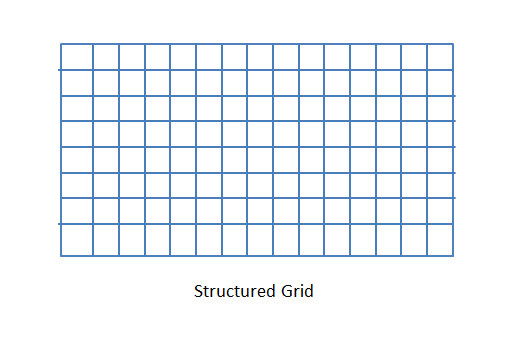
\includegraphics[width=5cm]{images/meshes/structured_grid}
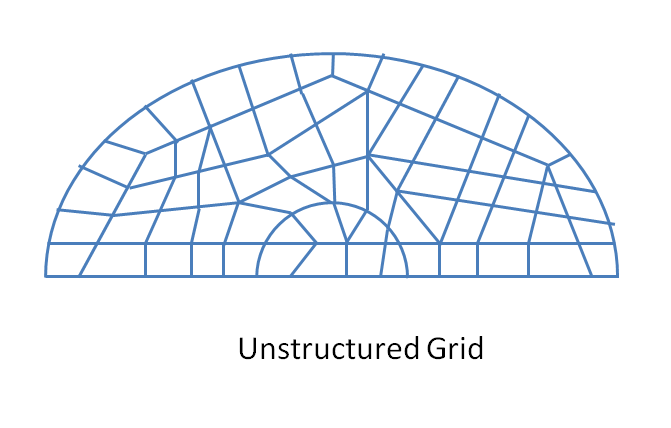
\includegraphics[width=5cm]{images/meshes/unstructured_grid}
\end{center}

\begin{remark}
\index{general}{Meshless}
Various families of so-called meshless methods exist and are commonly employed in Computational 
Fluid Dynamics \cite{liugu,liliu,grliu,liuliu}. They are however very rarely used in 
Computational geodynamics, with a noticeable exception \cite{hans03}.
\end{remark}

%............................................
\subsubsection{Quadrilateral-based meshes}

Let us now focus on the case of a rectangular computational domain of size 
{\tt Lx} $\times$ {\tt Ly} with a regular mesh composed of {\tt nelx}$\times${\tt nely}={\tt nel}
   quadrilaterals.  
There are then {\tt nnx}$\times${\tt nny}={\tt nnp} grid points.
The elements are of size {\tt hx}$\times${\tt hy} with {\tt hx}={\tt Lx}/{\tt nelx}.

We have no reason to come up with an irregular/illogical node numbering so 
we can number nodes row by row or column by column as shown on the example 
hereunder of a 3$\times$2 grid:

\begin{verbatim}
8=======9======10======11       2=======5=======8======11
|       |       |       |       |       |       |       |
|  (3)  |  (4)  |  (5)  |       |  (1)  |  (3)  |  (5)  |
|       |       |       |       |       |       |       |
4=======5=======6=======7       1=======4=======7======10
|       |       |       |       |       |       |       |
|  (0)  |  (1)  |  (2)  |       |  (0)  |  (2)  |  (4)  |
|       |       |       |       |       |       |       |
0=======1=======2=======3       0=======3=======6=======9

     "row by row"                  "column by column"
\end{verbatim}

The numbering of the elements themselves could be done in a somewhat chaotic 
way but we follow the numbering of the nodes for simplicity.
The row by row option is the adopted one in \fieldstone{} and the coordinates of the 
points are computed as follows:

\begin{lstlisting}
x = np.empty(nnp, dtype=np.float64)
y = np.empty(nnp, dtype=np.float64)
counter = 0
for j in range(0,nny):
    for i in range(0,nnx):
        x[counter]=i*hx
        y[counter]=j*hy
        counter += 1
\end{lstlisting}
The inner loop has {\tt i} ranging from {\tt 0} to {\tt nnx-1} first for {\tt j}=0, 1, ...
up to {\tt nny-1} which indeed corresponds to the row by row numbering.

\index{general}{Connectivity Array} 
We now turn to the connectivity. As mentioned before, this is a structured mesh so that the so-called
connectivity array, named {\tt icon} in our case, can be filled easily. For each element we need
to store the node identities of its vertices. Since there are {\tt nel} elements and {\tt m=4} corners, 
this is a {\tt m}$\times${\tt nel} array. The algorithm goes as follows:

\begin{lstlisting}
icon =np.zeros((m,nel),dtype=np.int16)
counter = 0
for j in range(0,nely):
    for i in range(0,nelx):
        icon[0,counter] = i + j * nnx 
        icon[1,counter] = i + 1 + j * nnx 
        icon[2,counter] = i + 1 + (j + 1) * nnx 
        icon[3,counter] = i + (j + 1) * nnx 
        counter += 1
\end{lstlisting}

In the case of the 3$\times$2 mesh, the {\tt icon} is filled as follows:
\begin{center}
\begin{tabular}{ccccccc}
element id$\rightarrow$ &0 &1&2&3&4&5 \\
node id$\downarrow$ \\
0& 0& 1& 2& 4& 5  &6\\
1& 1& 2& 3& 5& 6  &7\\
2& 5& 6& 7& 9& 10 &11\\
3& 4& 5& 6& 8& 9  &10\\
\end{tabular}
\end{center}
It is to be understood as follows: element $\#4$ is composed of nodes 5, 6, 10 and 9.
Note that nodes are always stored in a counter clockwise manner, starting at the bottom left.
This is very important since the corresponding basis functions and their derivatives 
will be labelled accordingly.

In three dimensions things are very similar. The mesh now counts 
{\tt nelx}$\times${\tt nely}$\times${\tt nelz}={\tt nel} elements which represent 
a cuboid of size {\tt Lx}$\times${\tt Ly}$\times${\tt Lz}.
The position of the nodes is obtained as follows:
\begin{lstlisting}
x = np.empty(nnp,dtype=np.float64)
y = np.empty(nnp,dtype=np.float64)
z = np.empty(nnp,dtype=np.float64)
counter=0
for i in range(0,nnx):
    for j in range(0,nny):
        for k in range(0,nnz):
            x[counter]=i*hx
            y[counter]=j*hy
            z[counter]=k*hz
            counter += 1
\end{lstlisting}
The connectivity array is now of size {\tt m}$\times${\tt nel} with {\tt m=8}:
\begin{lstlisting}
icon =np.zeros((m,nel),dtype=np.int16)
counter = 0
for i in range(0,nelx):
    for j in range(0,nely):
        for k in range(0,nelz):
            icon[0,counter]=nny*nnz*(i  )+nnz*(j  )+k
            icon[1,counter]=nny*nnz*(i+1)+nnz*(j  )+k
            icon[2,counter]=nny*nnz*(i+1)+nnz*(j+1)+k
            icon[3,counter]=nny*nnz*(i  )+nnz*(j+1)+k
            icon[4,counter]=nny*nnz*(i  )+nnz*(j  )+k+1
            icon[5,counter]=nny*nnz*(i+1)+nnz*(j  )+k+1
            icon[6,counter]=nny*nnz*(i+1)+nnz*(j+1)+k+1
            icon[7,counter]=nny*nnz*(i  )+nnz*(j+1)+k+1
            counter += 1
\end{lstlisting}

\improvement[inline]{produce drawing of node numbering}

Although it is not very common in geosciences, quadrilateral meshes are sometimes 
employed in a boundary-fitted way, as shown hereunder:

\begin{center}
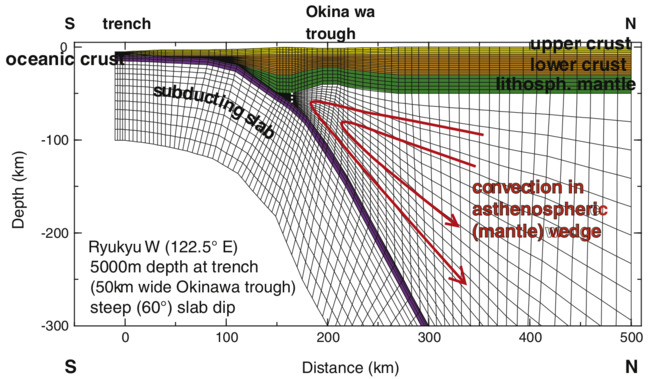
\includegraphics[width=7cm]{images/meshes/gukt16}\\
\end{center}


\Literature: \cite{jole97}

%...................................................
\subsubsection{Delaunay triangulation and Voronoi cells, and triangle-based meshes}

The topic of Delaunay\footnote{The triangulation is named after 
Boris Delaunay for his work on this topic from 1934.}
 triangulation is vast, but a simple definition can be written 
as follows:
"a Delaunay triangulation for a set P 
of points in a plane is a triangulation DT(P) such that no point in P is  
inside the circumcircle of any triangle in DT(P)." [wikipedia]
Other properties of such triangulations are that they 
maximize the minimum angle of all the angles of the 
triangles in the triangulation.
Note that for four or more 
points on the same circle (e.g., the vertices of a rectangle) the Delaunay triangulation is  
not unique and that points on a line also cannot yield a valid triangulation
(for the simple reason that they do not form a triangle).

\begin{center}
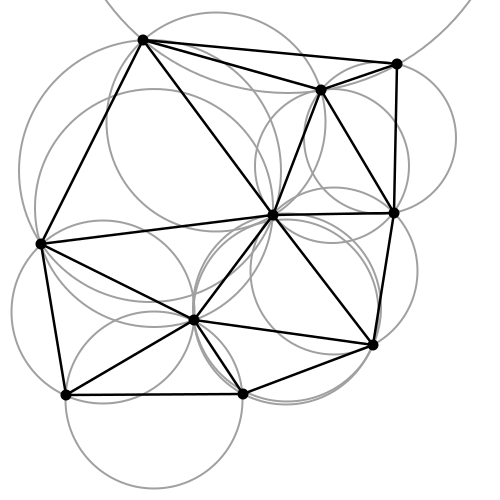
\includegraphics[width=4cm]{images/meshes/delaunay}
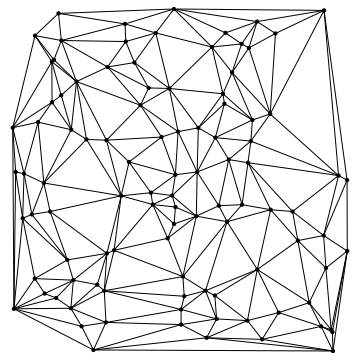
\includegraphics[width=4cm]{images/meshes/delaunay3}\\
{\captionfont a) A Delaunay triangulation in the plane with circumcircles shown.
b) The Delaunay triangulation of a random set of 100 points in a plane.}
\end{center}

The Delaunay triangulation of a discrete point set P in general corresponds 
to the dual graph of the Voronoi diagram for P. 
A Voronoi diagram is composed of non-overlapping Voronoi cells which make a partition 
of the plane. 
For each point there is a corresponding region consisting of all points closer to that 
point than to any other: this region is the Voronoi cell of that point.

\begin{center}
a)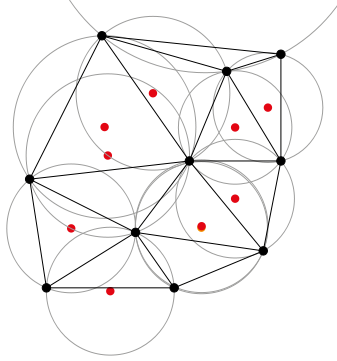
\includegraphics[width=4cm]{images/meshes/delaunay2}
b)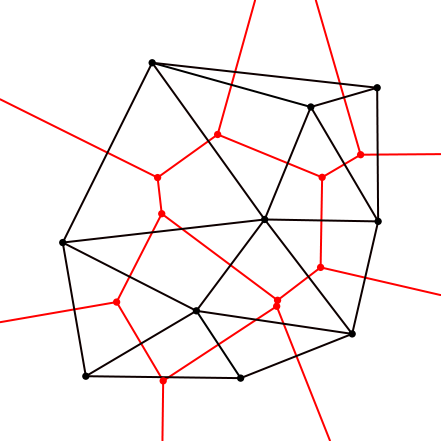
\includegraphics[width=4cm]{images/meshes/voronoi}\\
{\captionfont a) The Delaunay triangulation with all the circumcircles and their centers (in red).
b) Connecting the centers of the circumcircles produces the Voronoi diagram (in red). }
\end{center}

The Delaunay triangulation is used in the \douar code which is based on a particle levelset function to track materials. These particles are connected by means of a Delaunay triangulation (usually in a plane at startup, and then in a local Euclidean geometry once the surface is deformed) \cite{brtf08}.

\Literature: \cite{gebo}.


Once a Delaunay triangulation has been obtained it can be used as a FEM mesh.  
Triangle-based meshes are obviously better suited for simulations of complex geometries:
\begin{center}
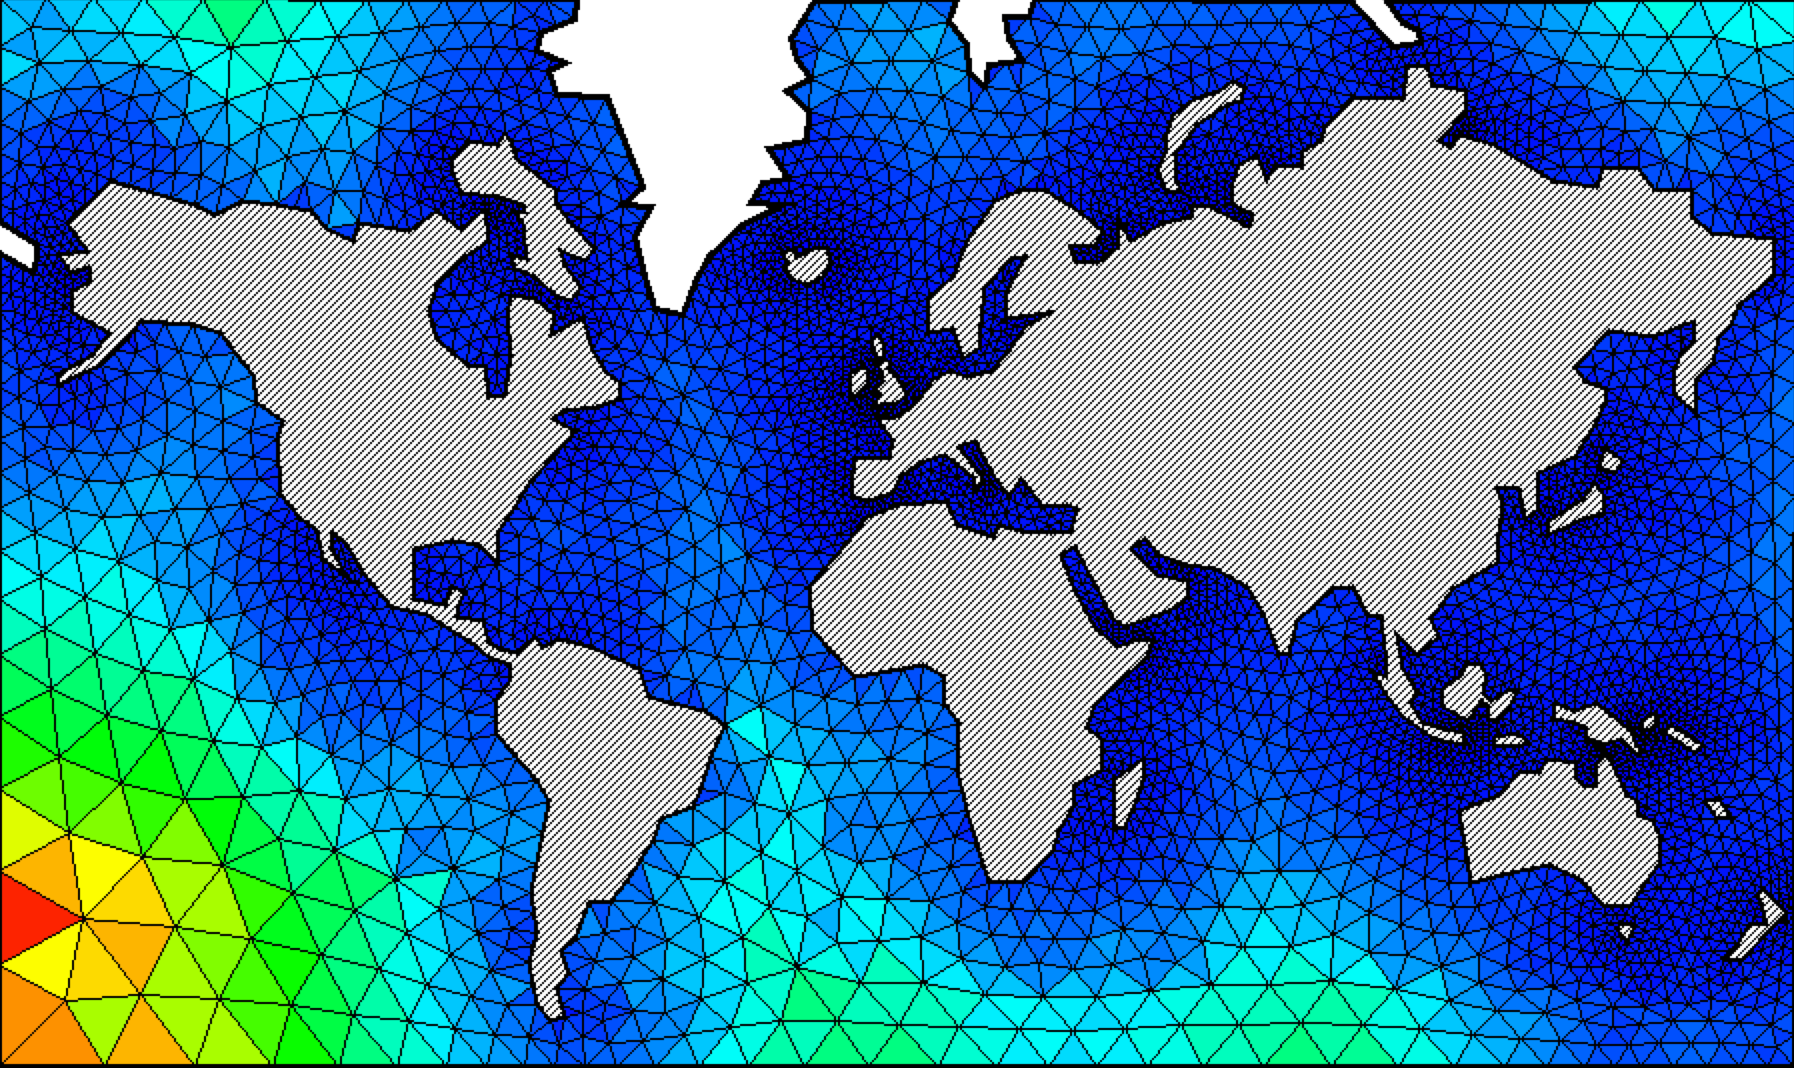
\includegraphics[height=4cm]{images/meshes/tr1}
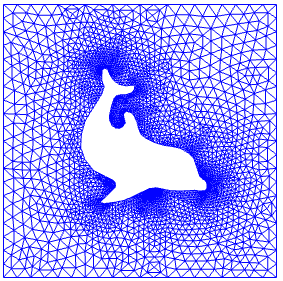
\includegraphics[height=4cm]{images/meshes/dolfin}\\
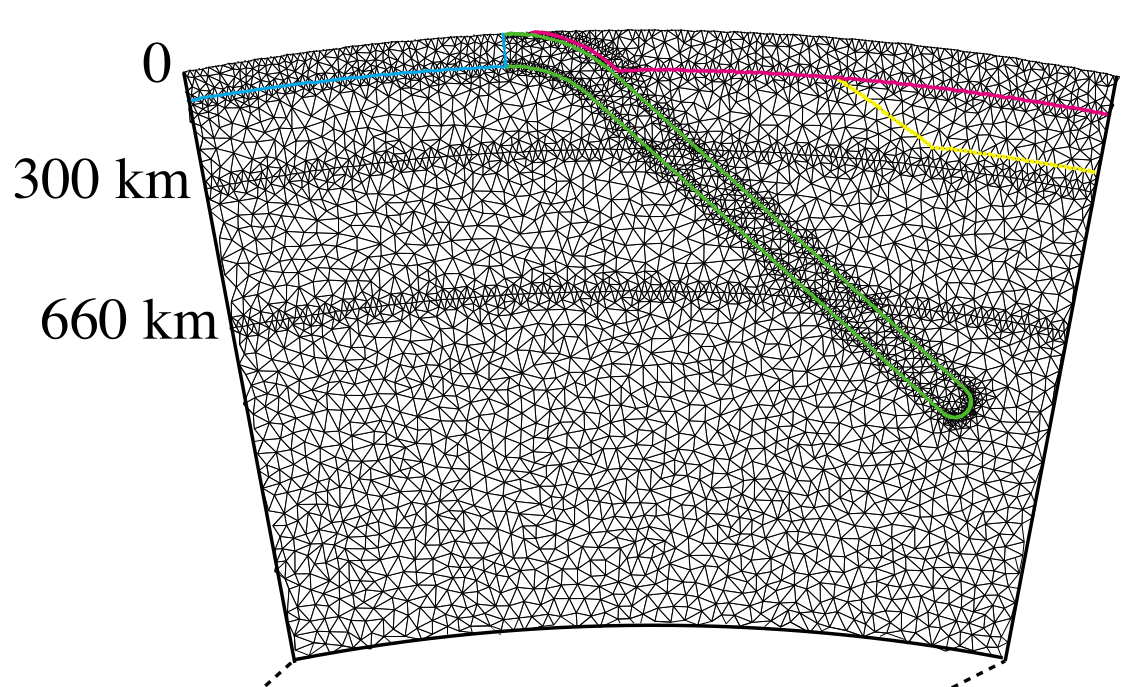
\includegraphics[height=3.8cm]{images/meshes/gebk12}\cite{gebk12}
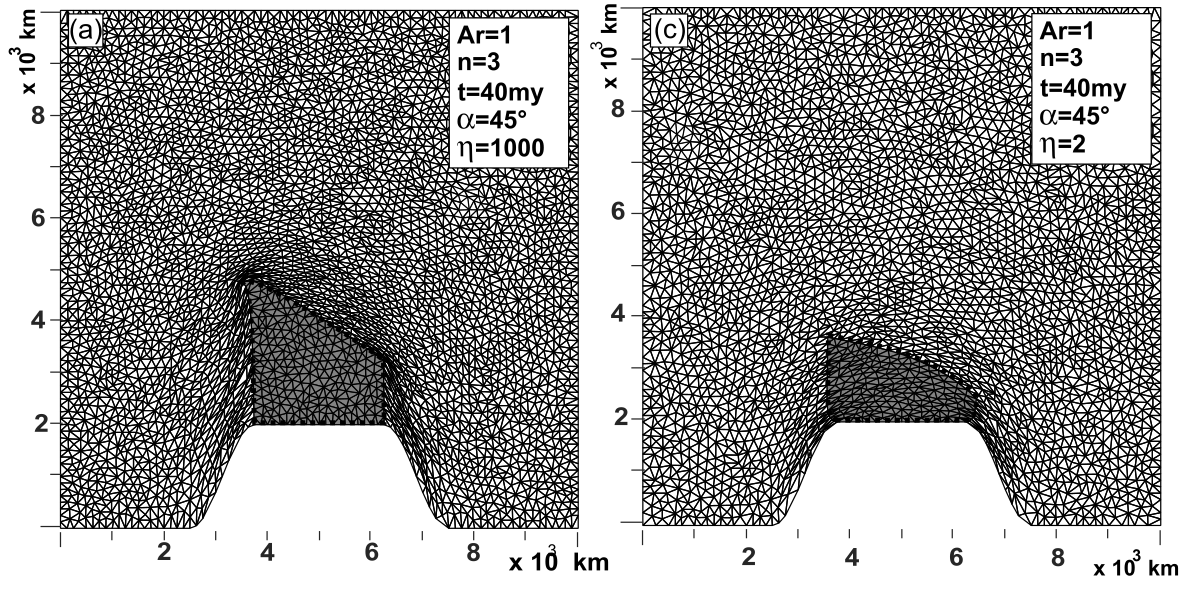
\includegraphics[height=3.8cm]{images/meshes/rost05a}\cite{rost05a}
\end{center}

A very practical 2D triangle mesher is the 
code {\sl Triangle}\footnote{\url{https://www.cs.cmu.edu/~quake/triangle.html}}
written by J.R. Shewchuk \cite{shew96,shew02,shew14}.
Triangle is specialized for creating two-dimensional finite element meshes, but can 
also perform simpler related tasks such as forming Delaunay triangulations under various assumptions.
Another very common mesher tool is Gmsh \cite{gere09}.

\begin{center}
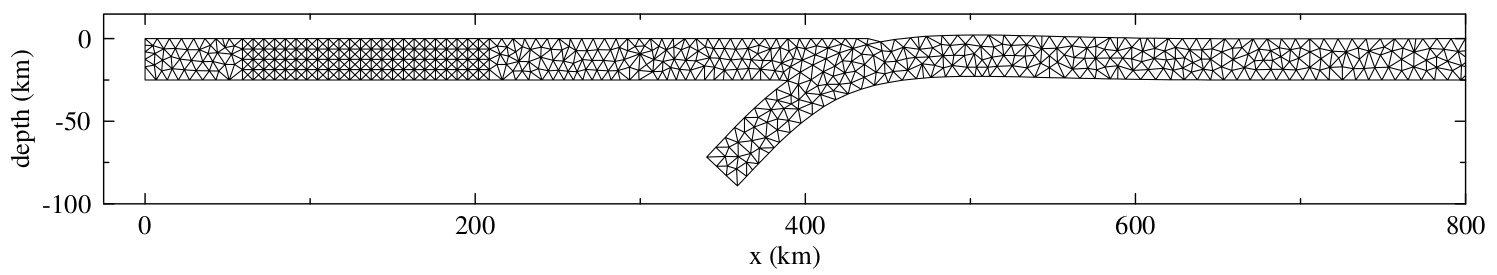
\includegraphics[width=13cm]{images/meshes/bugw01}\\
{\captionfont Taken from Buiter \etal \cite{bugw01}. Finite element grid. 
The subducting plate initially extends to 1226 km in the horizontal direction and 
is not completely shown here. Discretization in the subducting plate is slightly coarser 
towards the right edge.}
\end{center}

\begin{center}
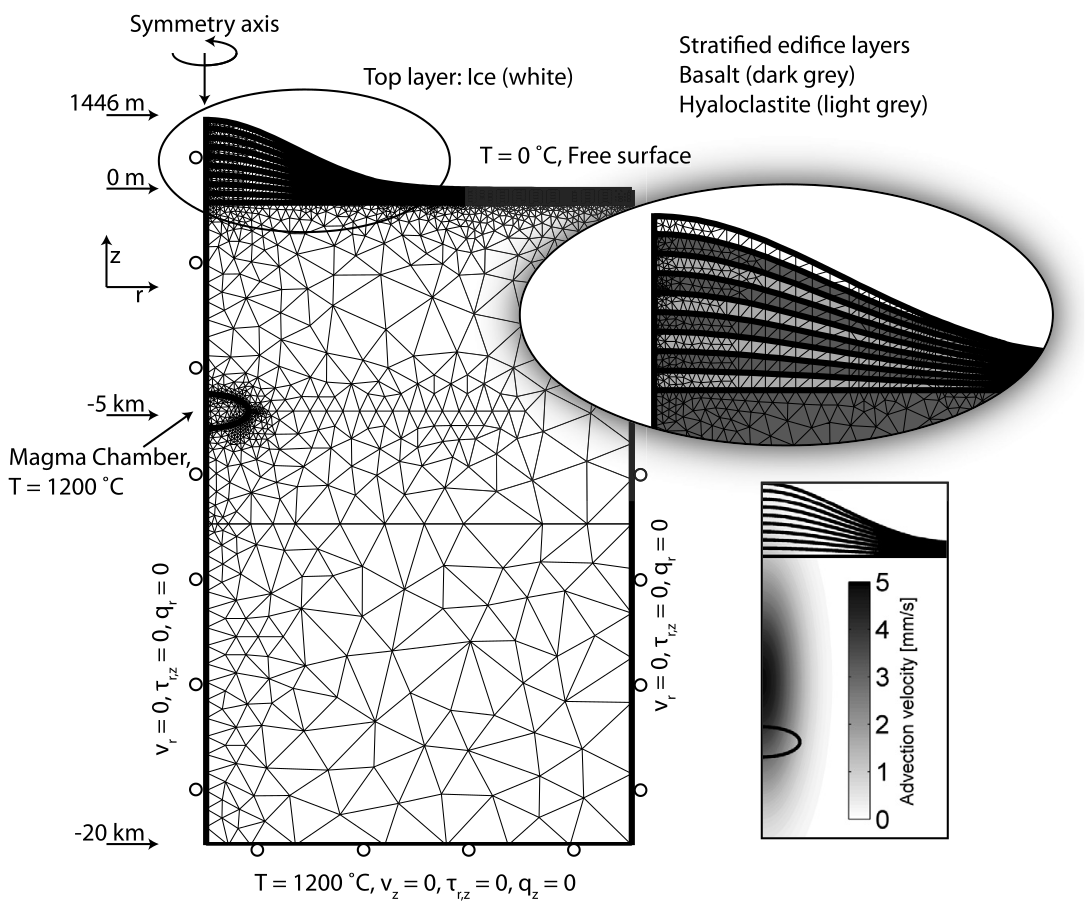
\includegraphics[width=13cm]{images/meshes/bafl16}\\
{\captionfont Numerical model setup of the 2D axisymmetric half-space with all applied 
boundary conditions to study the effects of ice-cap unloading
on shallow volcanic systems \cite{bafl16}}
\end{center}

\begin{center}
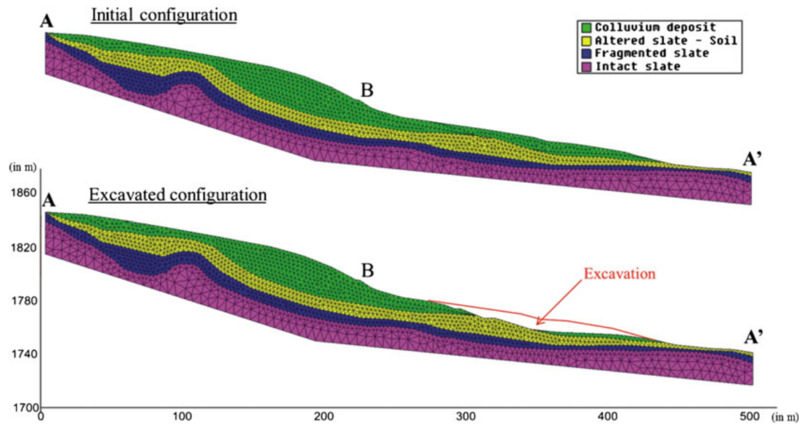
\includegraphics[width=13cm]{images/meshes/fegh14}\\
{\captionfont Taken from \cite{fegh14}. Modelling of slow
landslides. Finite element mesh in the initial and excavated configuration.}
\end{center}

Although it is rarely used in practice it is possible to produce meshes which contain 
both quadrilateral and triangular elements:
\begin{center}
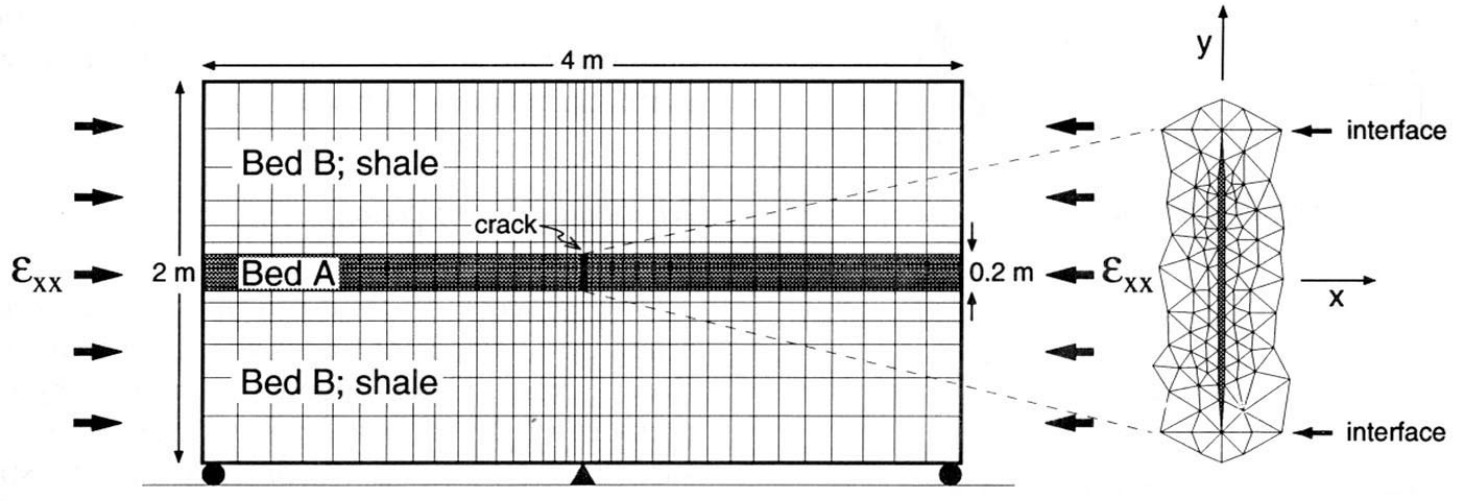
\includegraphics[width=13cm]{images/meshes/fige95}\\
{\captionfont Mesh used to analayse the stress distribution around a pressurized crack in a layered 
elastic medium \cite{fige95}}
\end{center}

\Literature \fullcite{musd15}\fullcite{vemm09}

\begin{remark} 
The Natural Neighbour Interpolation method of Sambridge \etal \cite{sabm95,sabm96} is based on the Delaunay triangulation.
\end{remark}

\begin{remark} 
Moresi \& Mather \cite{moma19} have released Stripy, a A Python module for (constrained) triangulation
in Cartesian coordinates and on a sphere, which is based on Stripack \cite{renk96,renk97}.
\end{remark}

\todo[inline]{write about gmesh}

\begin{center}
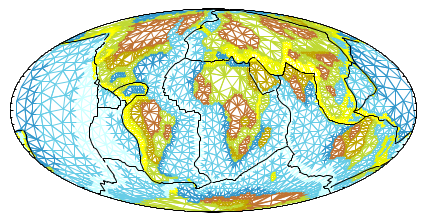
\includegraphics[width=6cm]{images/meshes/gusa98a}
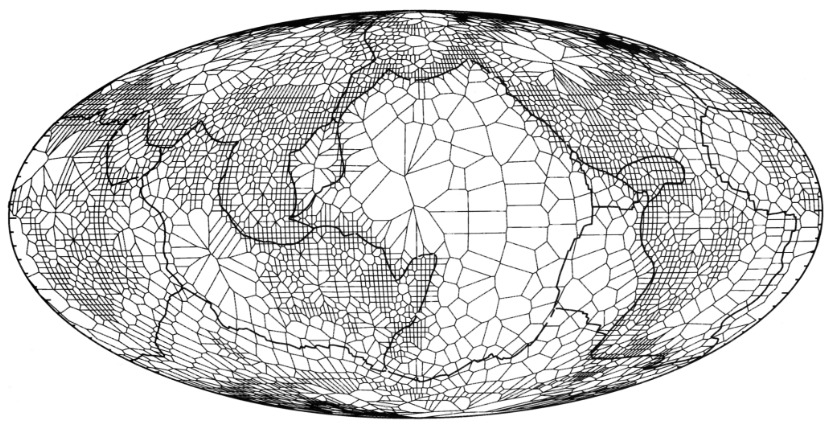
\includegraphics[width=6cm]{images/meshes/gusa98b}\\
{\captionfont Taken from Gudmundsson \& Sambridge (1998) \cite{gusa98}.
Boundaries of Voronoi cells around 4100 of the original 16,200 2x2 degree cells
selected to sample the details of the regionalization.}
\end{center}


%...........................
\subsubsection{Tetrahedra}

\begin{center}
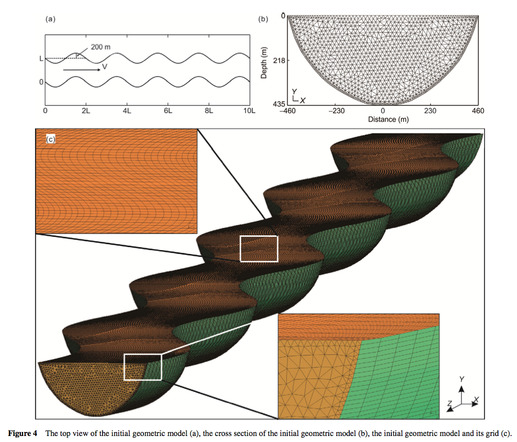
\includegraphics[width=5cm]{images/meshes/glacier}
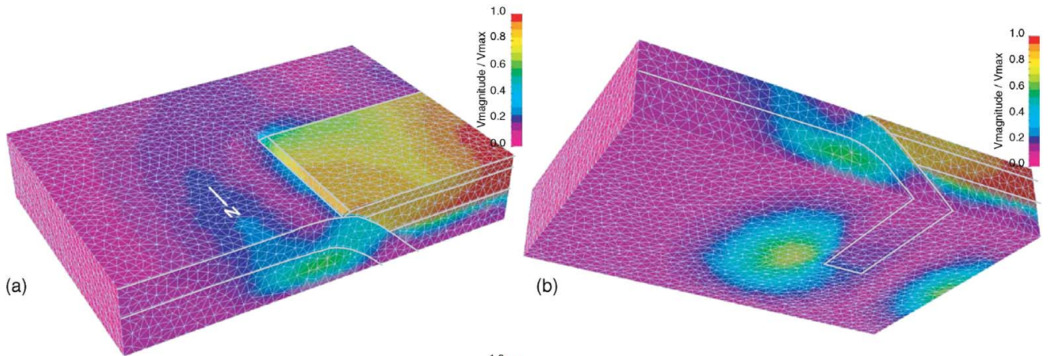
\includegraphics[width=10cm]{images/meshes/gowo05}\\
{\captionfont 
Left: Example of 3D mesh \textcite{yash15} (2015);
Right: Normalized velocities of a STEP subduction model \textcite{gowo05} (2005).
}
\end{center}

\begin{center}
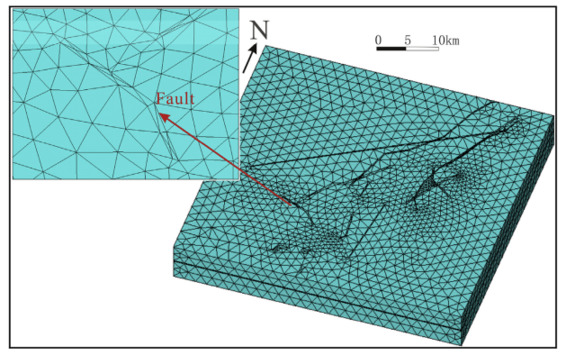
\includegraphics[width=7cm]{images/meshes/guyr16}
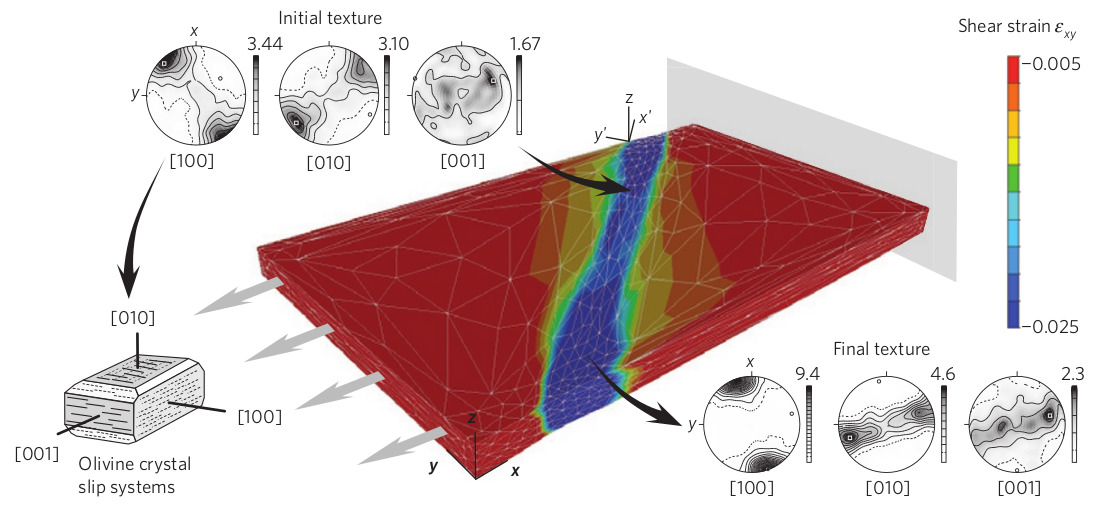
\includegraphics[width=8cm]{images/meshes/tokv09}\\
{\captionfont 
Left: 3D finite element grid in Damintun area, including prescribed faults, \textcite{guyr16} (2016);
Right: Structural reactivation in plate tectonics controlled by olivine crystal anisotropy, \textcite{tokv09} (2009).
}
\end{center}

\begin{center}
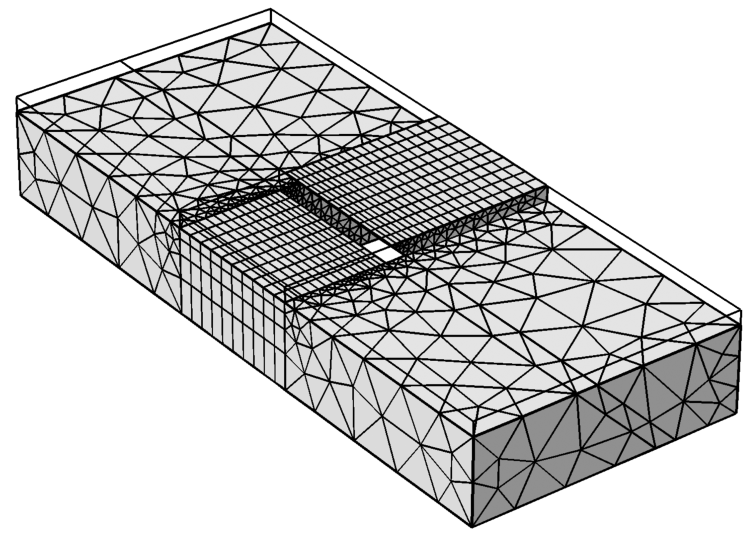
\includegraphics[width=6cm]{images/meshes/paml14b}
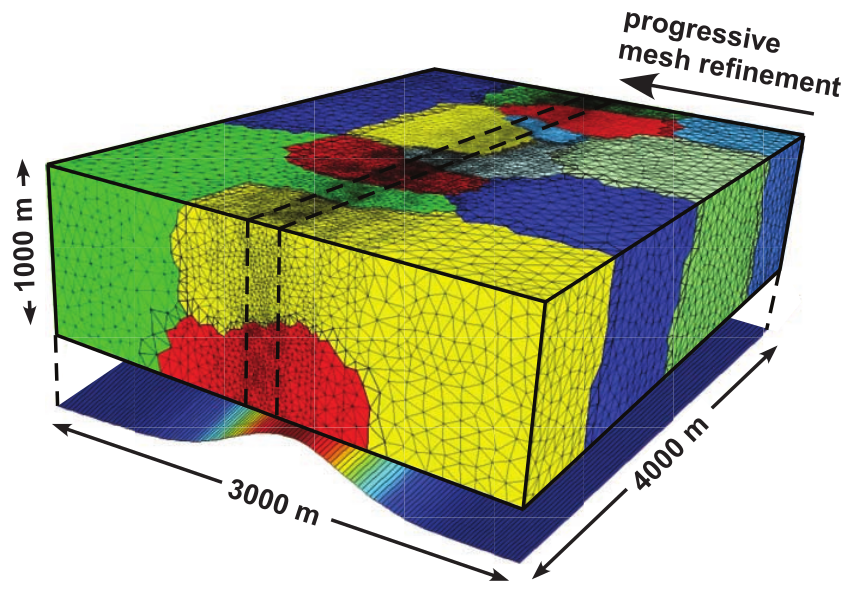
\includegraphics[width=6.3cm]{images/meshes/codh08}\\
{\captionfont 
Left: Mesh used for the three-dimensional model. A high resolution mesh is used in
the wedge and subslab domains, while the mesh resolution decays to lower values
toward the edge of the model. All elements are quadratic, allowing for twice the
resolution visualized here, \textcite{paml14b} (2014);
Right: Mid-Ocean Ridge Hydrothermal System: 3D mesh consisting of $2.5~\si{\meter}$ tetrahedron elements. 
Resolution is refined toward the axial center, with the finest resolution between the dashed
lines, and colors indicate computational domains assigned to separate processors, 
\textcite{codh08} (2008).}
\end{center}

\begin{center}
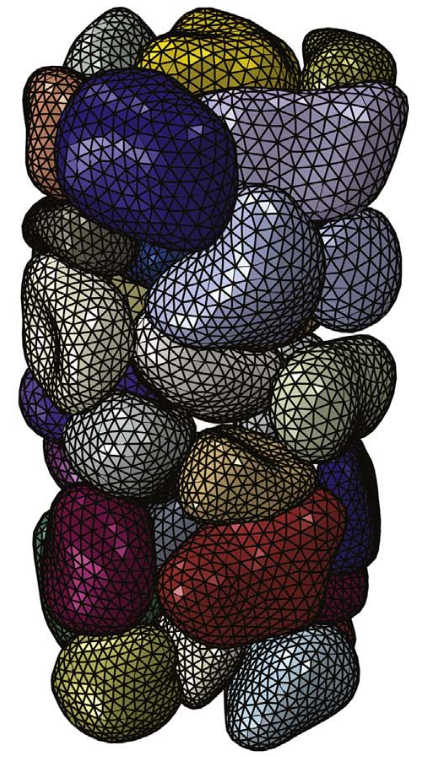
\includegraphics[width=3cm]{images/meshes/imal18}\\
{\captionfont Grains of sand before a compression experiment with FEM \textcite{imal18} (2018).}
\end{center}


Check TetGen mesher \fullcite{si15}. 

%............................................
\subsubsection{Hexahedra}

A hexahedron is a convex polytope isomorphic to the cube $[0,1]^3$.
Edges are line segments, facets are strictly {\bf planar} convex polygons.

\begin{center}
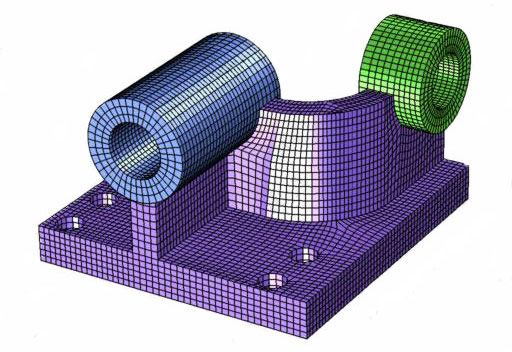
\includegraphics[width=5cm]{images/meshes/hexa.jpg}
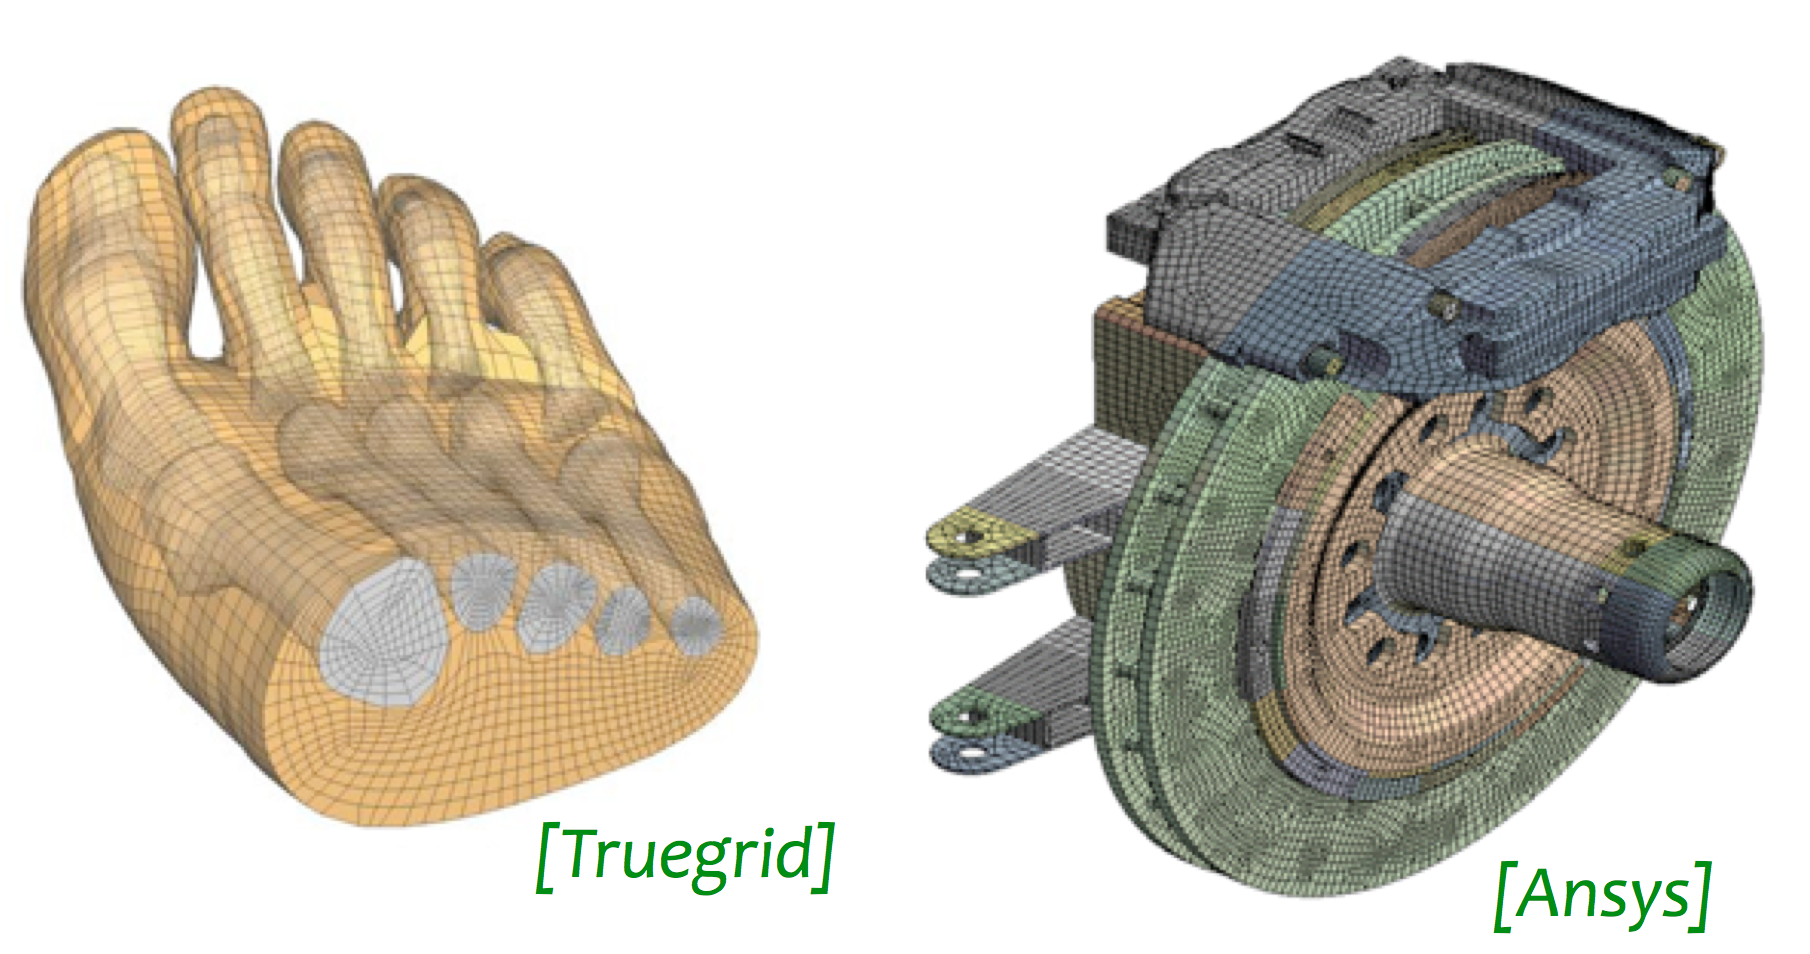
\includegraphics[width=6cm]{images/meshes/hexa2}
\end{center}

\Literature Efficient Volume computation for Three- Dimensional hexahedral Cells \cite{duko88,gran97}

%.......................................
\subsubsection{Adaptive Mesh Refinement}
\index{general}{AMR} \index{general}{Adaptive Mesh Refinement}

Let us do a simple calculation and assume we wish to model mantle convection on Earth. 
The inner radius is $R_1=$3485km and the bottom of the lithosphere is at $R_2=$6250km. 
The volume of fluid is then 
\[
V = \frac{4}{3}\pi (R_2^3-R_1^3) \simeq 8.5\times 10^{11} \text{km}^3
\]
Let us further assume that we are satisfied with an average resolution of 10km. 
Each element/cell is then $10^3\text{km}^3$ and the total number of elements/cell is then 
\[
N \simeq 8.5 \times 10^8 \sim {\cal O}(10^9)
\]
This is a very large number. The resulting linear systems from the discretisation of the 
equations on such a mesh will be very even larger for the Stokes equations and solving 
these systems will require very large numbers of CPUs and long compute times. 

Aside from these considerations it is quite obvious that a high resolution mesh is not needed 
in parts of the mantle where large scale upwellings and downwellings occur, but 
probably even higher resolution will be needed in the vicinity of thin plumes and boundary layers. 
This means that a uniform mesh is a sub-optimal way of discretising space for such problems. 

The same reasoning also holds in the lithosphere where for instance narrow plate boundaries need to 
be adequately resolved while the inside of rigid plates can be modelled with coarser meshes. 

Finally, although one could employ meshing software to arrive at well balanced meshes in space, the 
dynamic character of the geodynamics modelling renders this approach cumbersome. A subduction zone, 
a mid-ocean rift or an ascending plume will evolve in time and the mesh will have to evolve in time too. 

In light of all this, it was only a matter of time before Adaptive Mesh Refinement was adopted 
in computatinal geodynamics. However, since the use and update of such meshes is somewhat 
complex in terms of numerical algorithms, its introduction came somewhat late (00's and later).
The \douar code (see Section~\ref{app:codes}) developed originally by J. Braun and Ph. Fullsack 
is a prime example of an early multi-purpose code relying on a self-written Octree library \cite{brtf08}.
More recently the \aspect{} code was developed on top of the Octree library p4est \cite{buwg11}

For further reading I suggest you read the review by May, Schellart \& Moresi on this topic \cite{masm13}.

\begin{center}
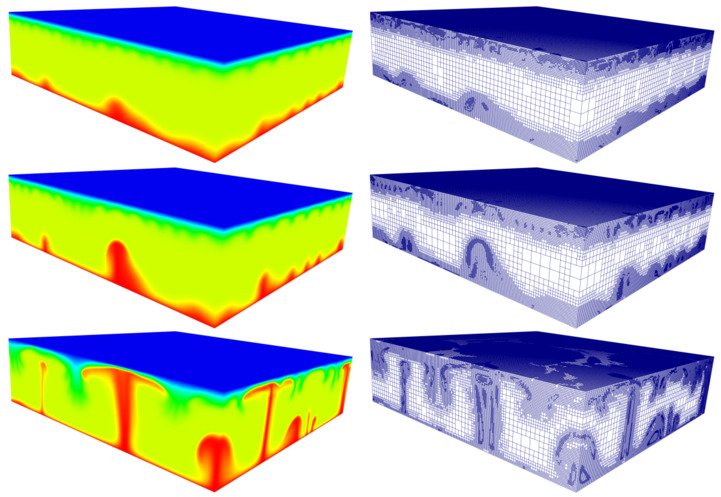
\includegraphics[height=6cm]{images/meshes/bugg08.jpg}
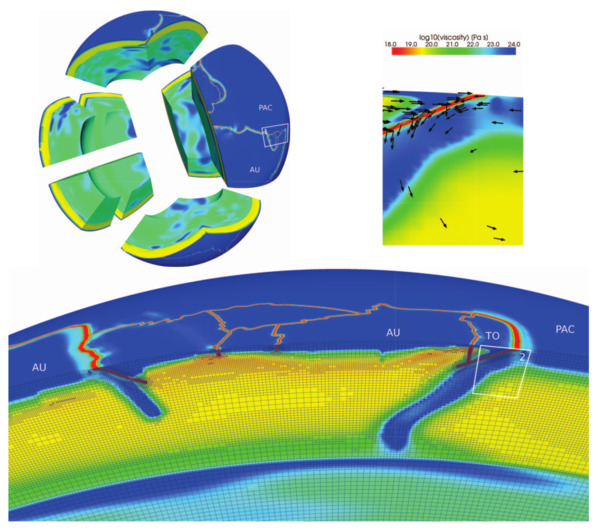
\includegraphics[height=6cm]{images/meshes/bugg10.jpg}\\
{\captionfont Taken from \cite{bugg08} and \cite{bugg10}}
\end{center}

\begin{center}
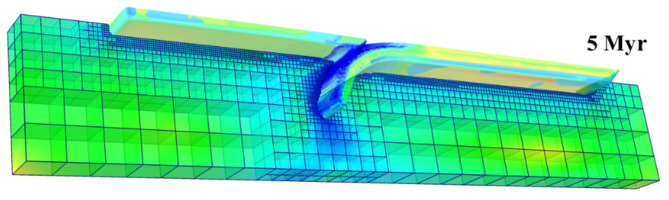
\includegraphics[height=3.8cm]{images/meshes/gltf18.jpg}\\
{\captionfont Taken from \cite{gltf18}}
\end{center}


\Literature: \cite{bugg08,bugg10}\cite{lezh11} \cite[sect 3]{bugs09} \cite{dadh07}
\cite{svna18} \cite{mish11}


\newpage
\paragraph{A short illustrative exercise}.


\noindent 
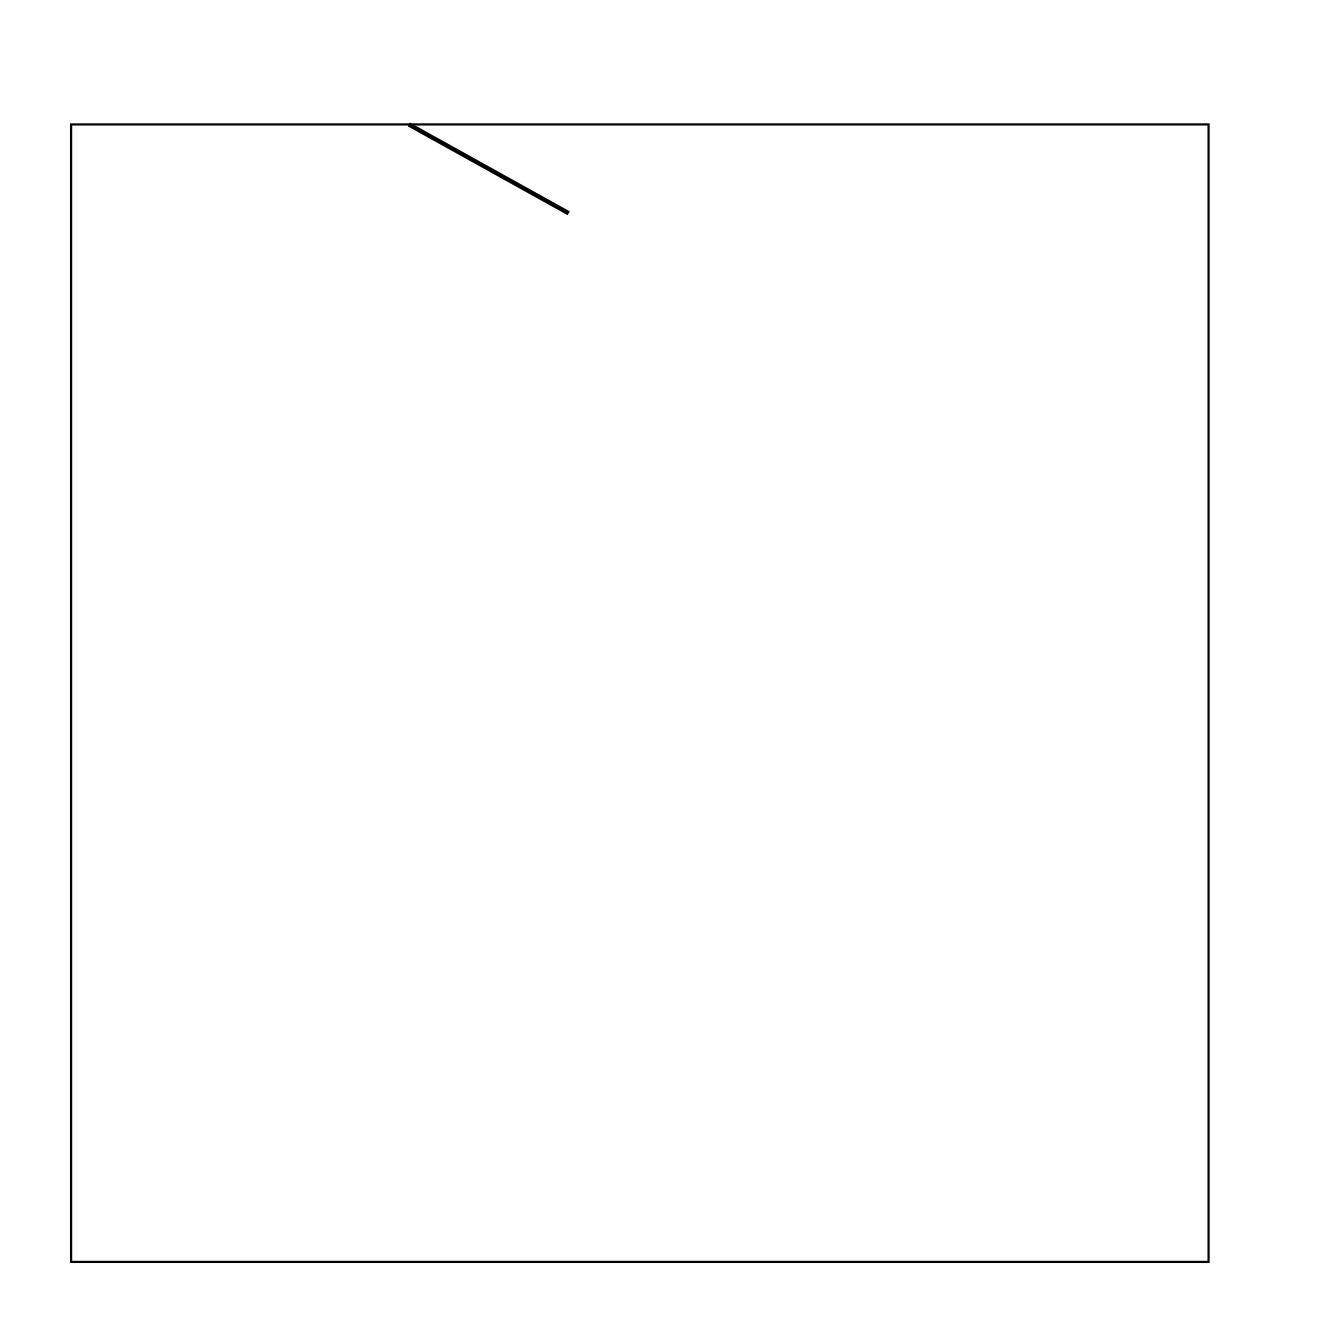
\includegraphics[width=4.5cm]{images/meshes/AMR/amr0}
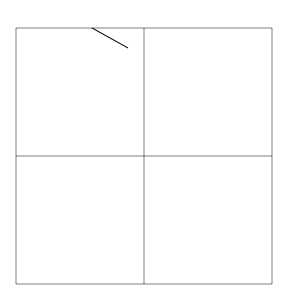
\includegraphics[width=4.5cm]{images/meshes/AMR/amr1}
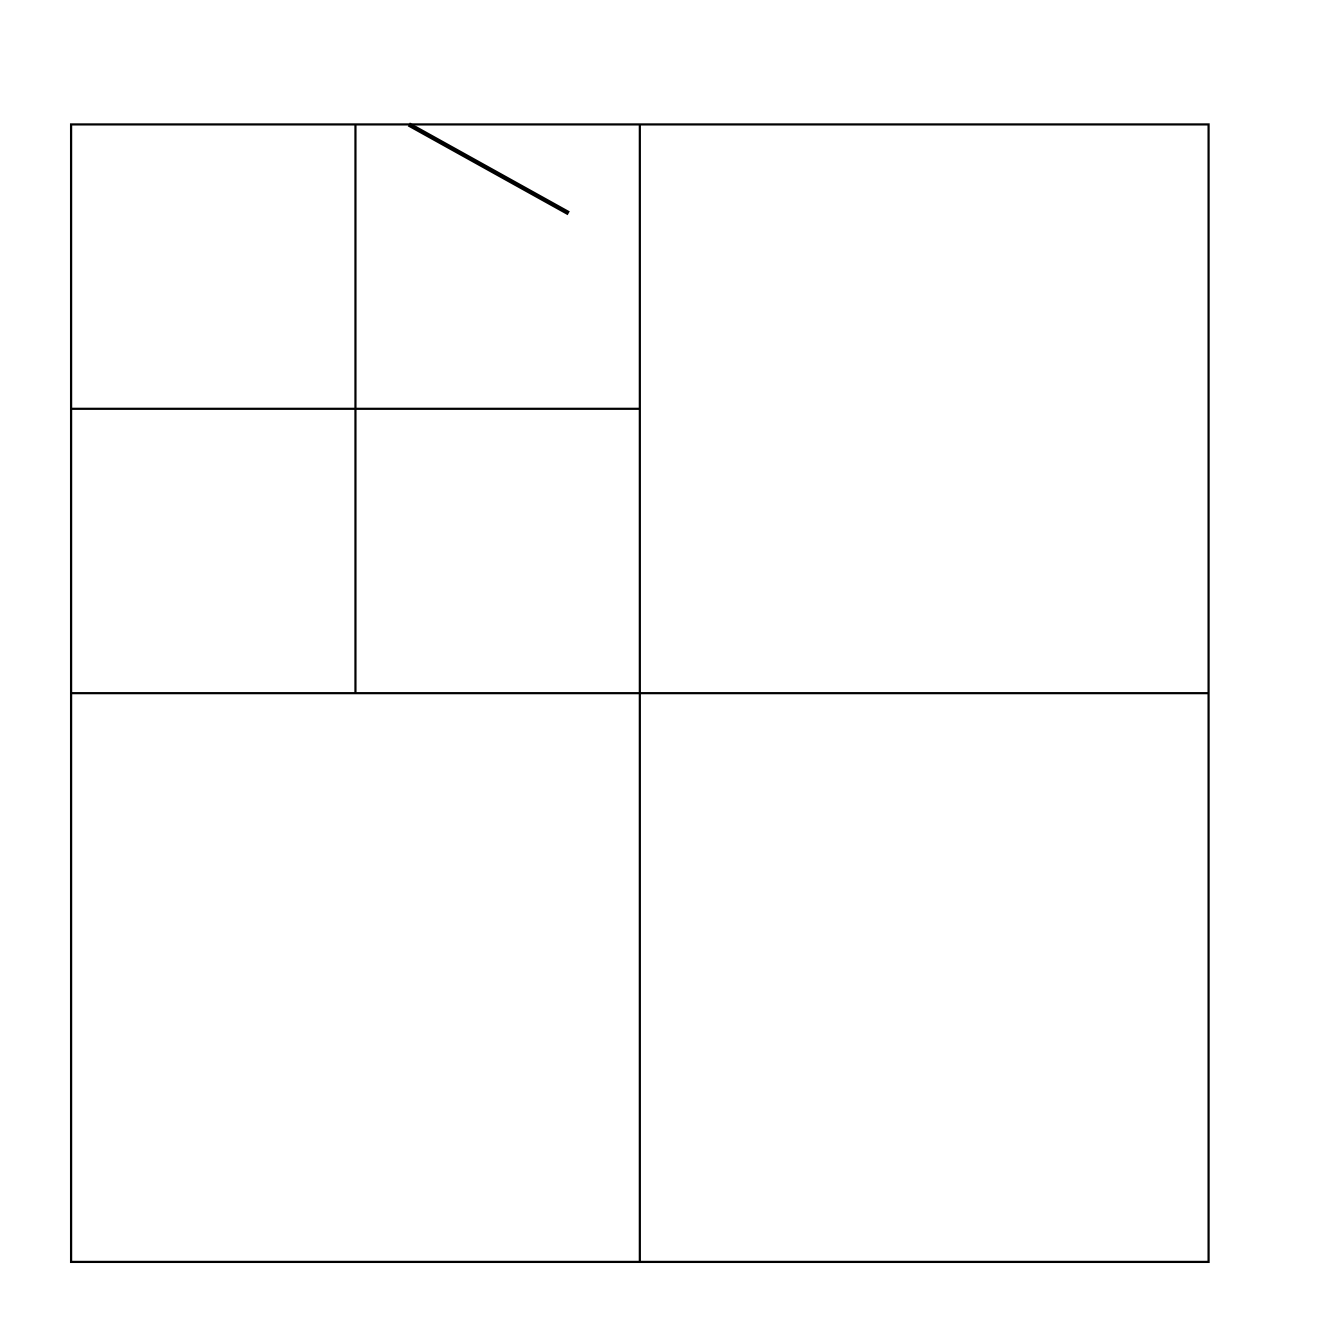
\includegraphics[width=4.5cm]{images/meshes/AMR/amr2}\\
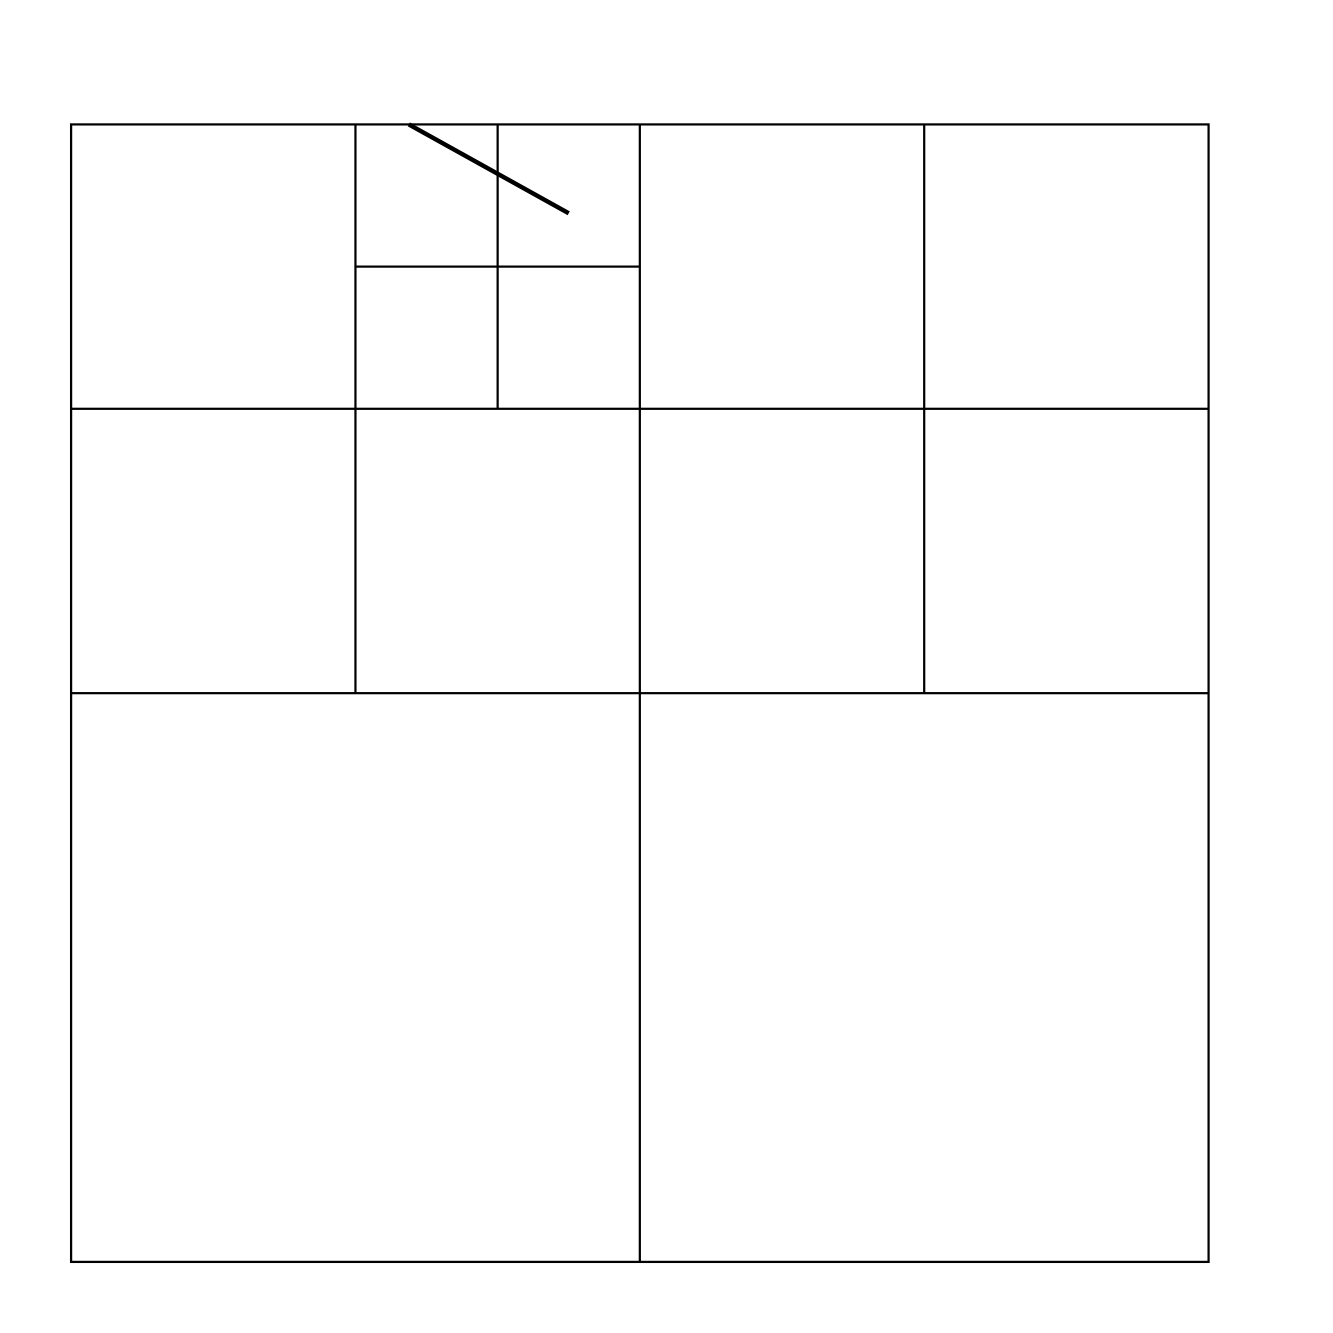
\includegraphics[width=4.5cm]{images/meshes/AMR/amr3}
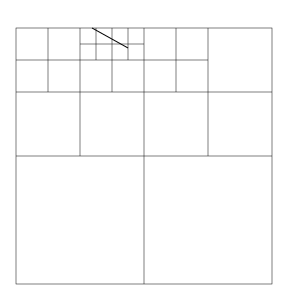
\includegraphics[width=4.5cm]{images/meshes/AMR/amr4}
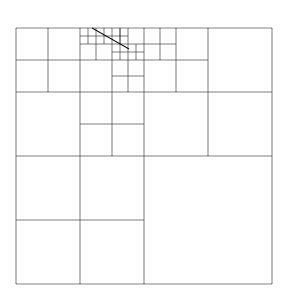
\includegraphics[width=4.5cm]{images/meshes/AMR/amr5}\\
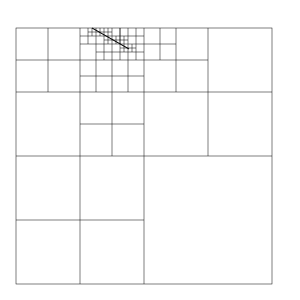
\includegraphics[width=4.5cm]{images/meshes/AMR/amr6}
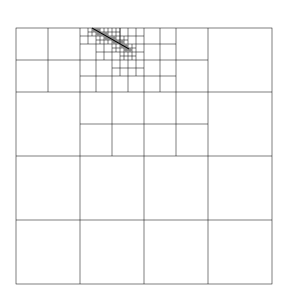
\includegraphics[width=4.5cm]{images/meshes/AMR/amr7}
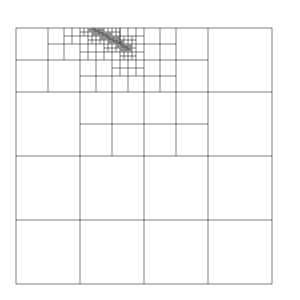
\includegraphics[width=4.5cm]{images/meshes/AMR/amr8}

\begin{tabular}{l|ccccccccc}
             & \# l0  & \# l1 & \# l2 & \# l3 & \# l4 & \# l5 & \# l6 & \# l7 & \# l8 \\ 
\hline\hline
max level= 0 & 1 & \\
max level= 1 & 0 & 4 & \\
max level= 2 & 0 & 3 & 4 \\
max level= 3 & 0 & 2 & 7 & 4\\
max level= 4 & 0 & 2 & 5 & 10 & 8 \\
max level= 5 & 0 & 1 & 8 & 12 & 11 & 20 \\ 
max level= 6 & 0 & 1 & 8 & 11 & 13 & 20 & 32 \\
max level= 7 & 0 & 0 & 11 & 14 & 15 & 23 & 37 & 60 \\
max level= 8 & 0 & 0 & 11 & 13 & 17 & 27 & 43 & 72 & 116 \\
\hline
\end{tabular}

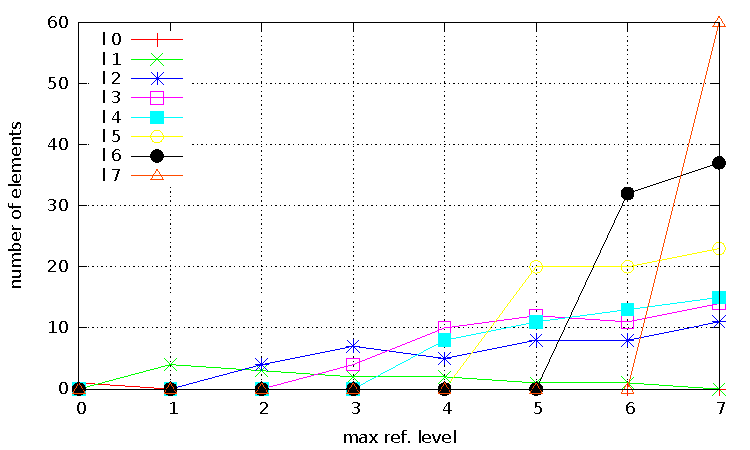
\includegraphics[width=7.28cm]{images/meshes/AMR/amr_data1.pdf}
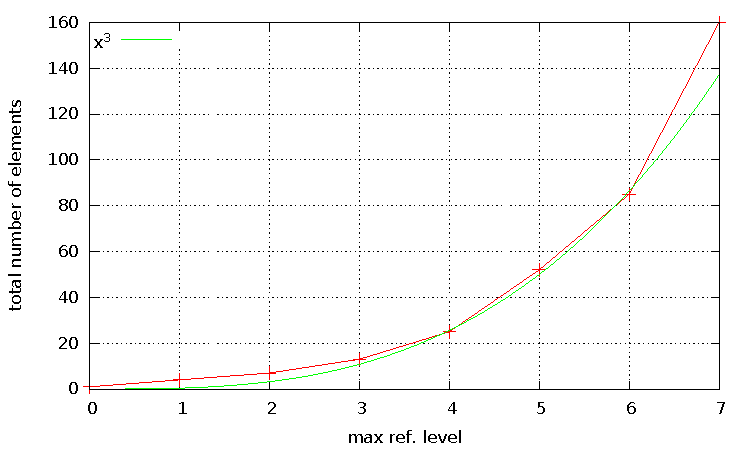
\includegraphics[width=7.28cm]{images/meshes/AMR/amr_data2.pdf}

In the particular case presented here, even though the inclusion in a short 
two-dimensional line, the total number of elements grows faster than the 
third power of the refinement level. While of course the total number 
of elements remains much smaller than the constant resolution counterpart, 
this observation tells us that authorising a unit increase of the maximum 
refinement level can have a substantial effect on the total number of elements.

\newpage

\noindent
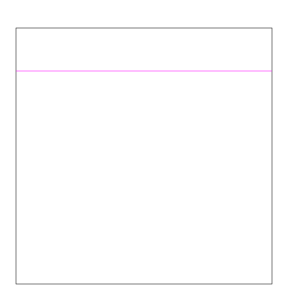
\includegraphics[width=4cm]{images/meshes/AMR/amr_0}
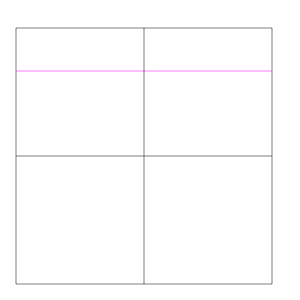
\includegraphics[width=4cm]{images/meshes/AMR/amr_1}
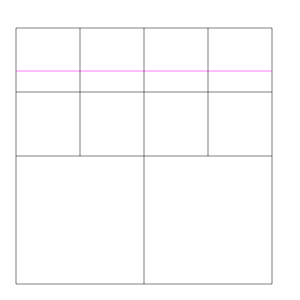
\includegraphics[width=4cm]{images/meshes/AMR/amr_2}
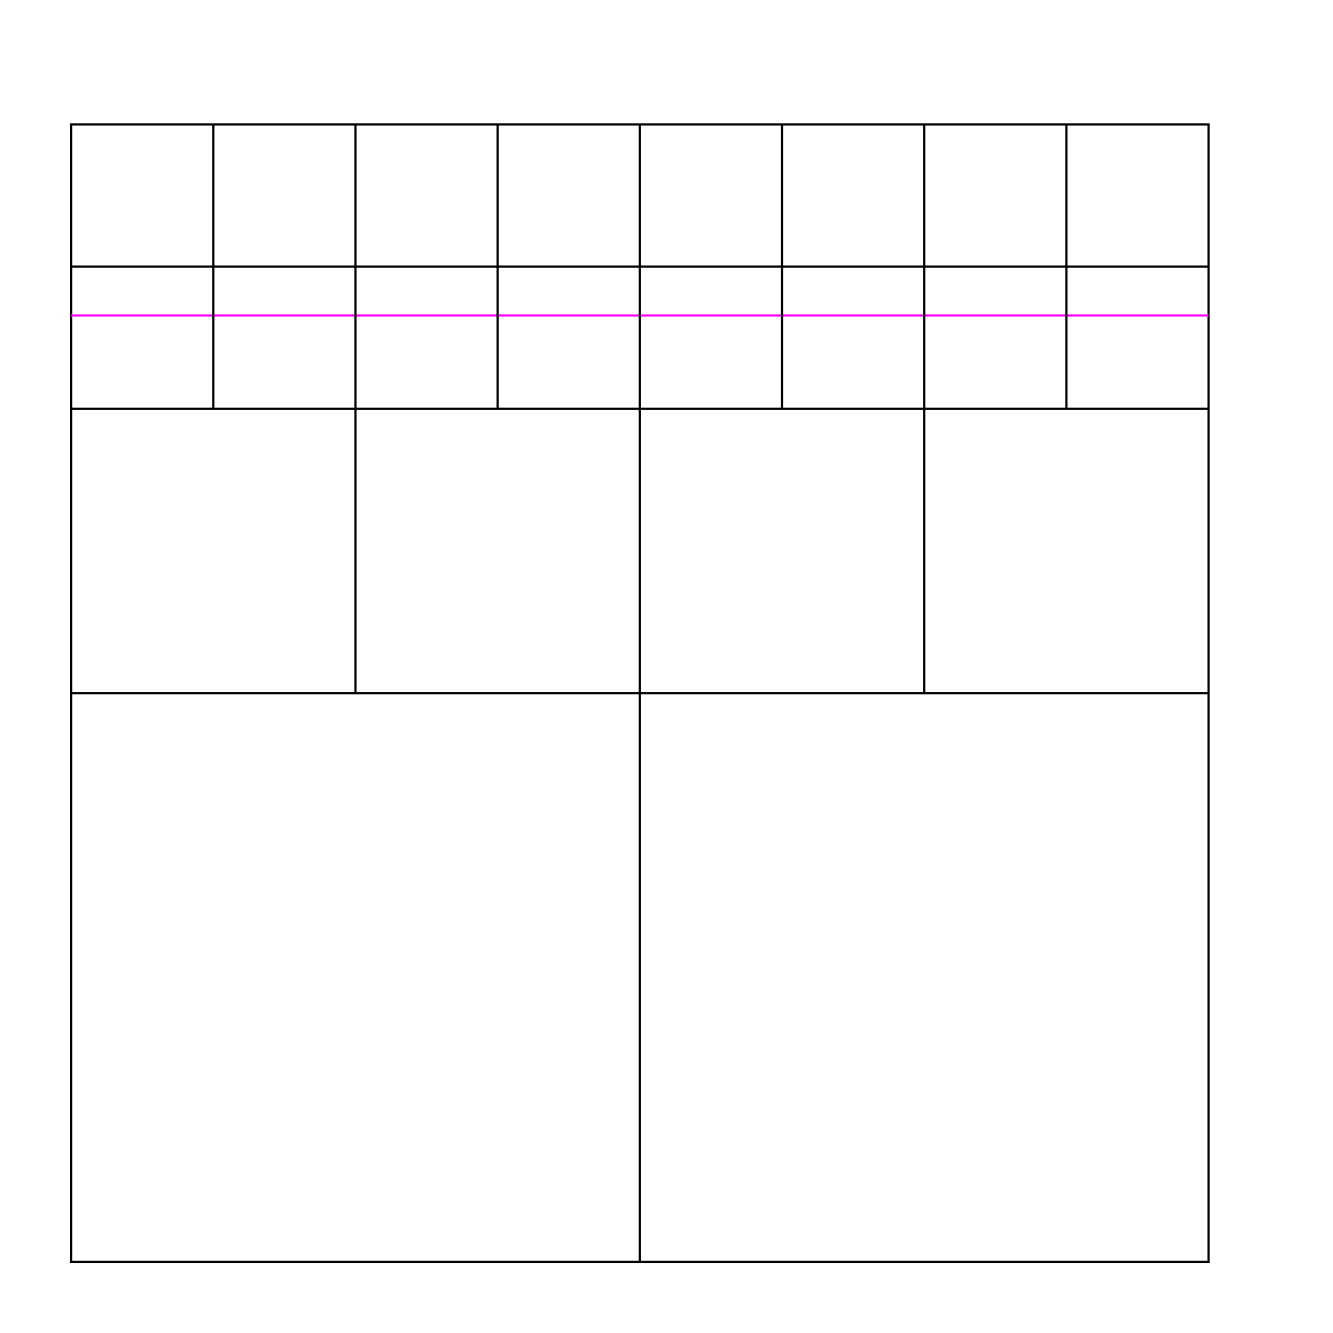
\includegraphics[width=4cm]{images/meshes/AMR/amr_3}\\
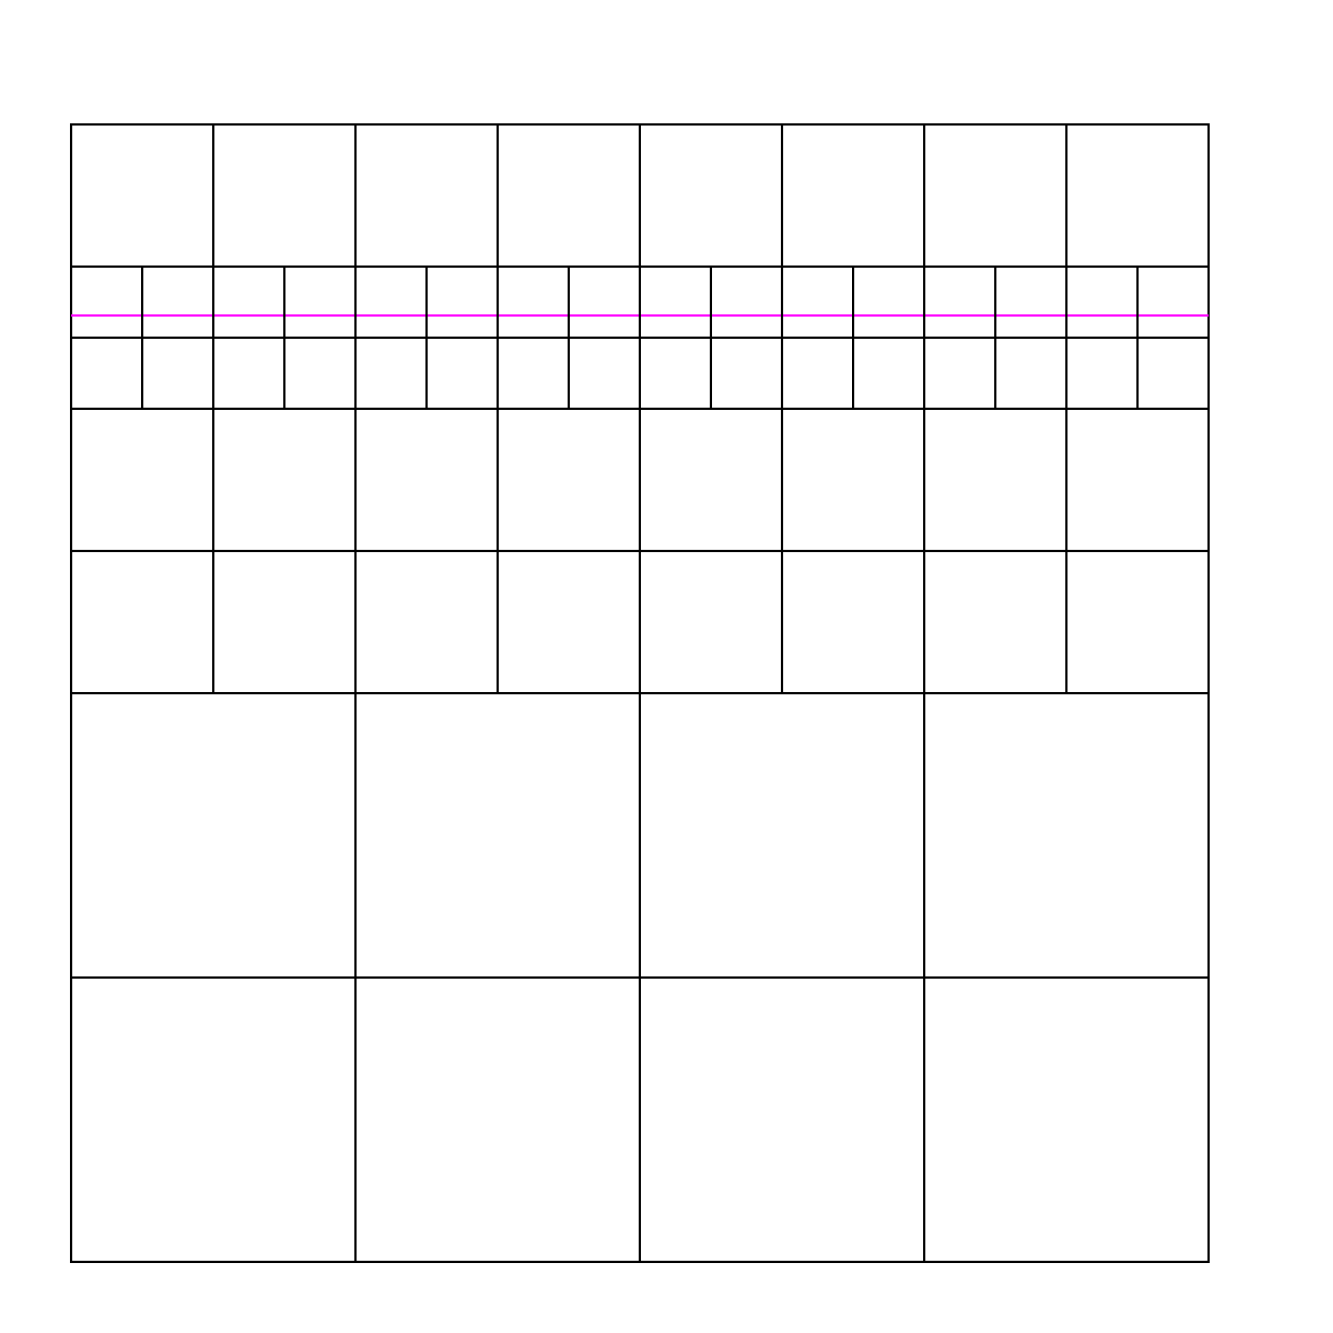
\includegraphics[width=4cm]{images/meshes/AMR/amr_4}
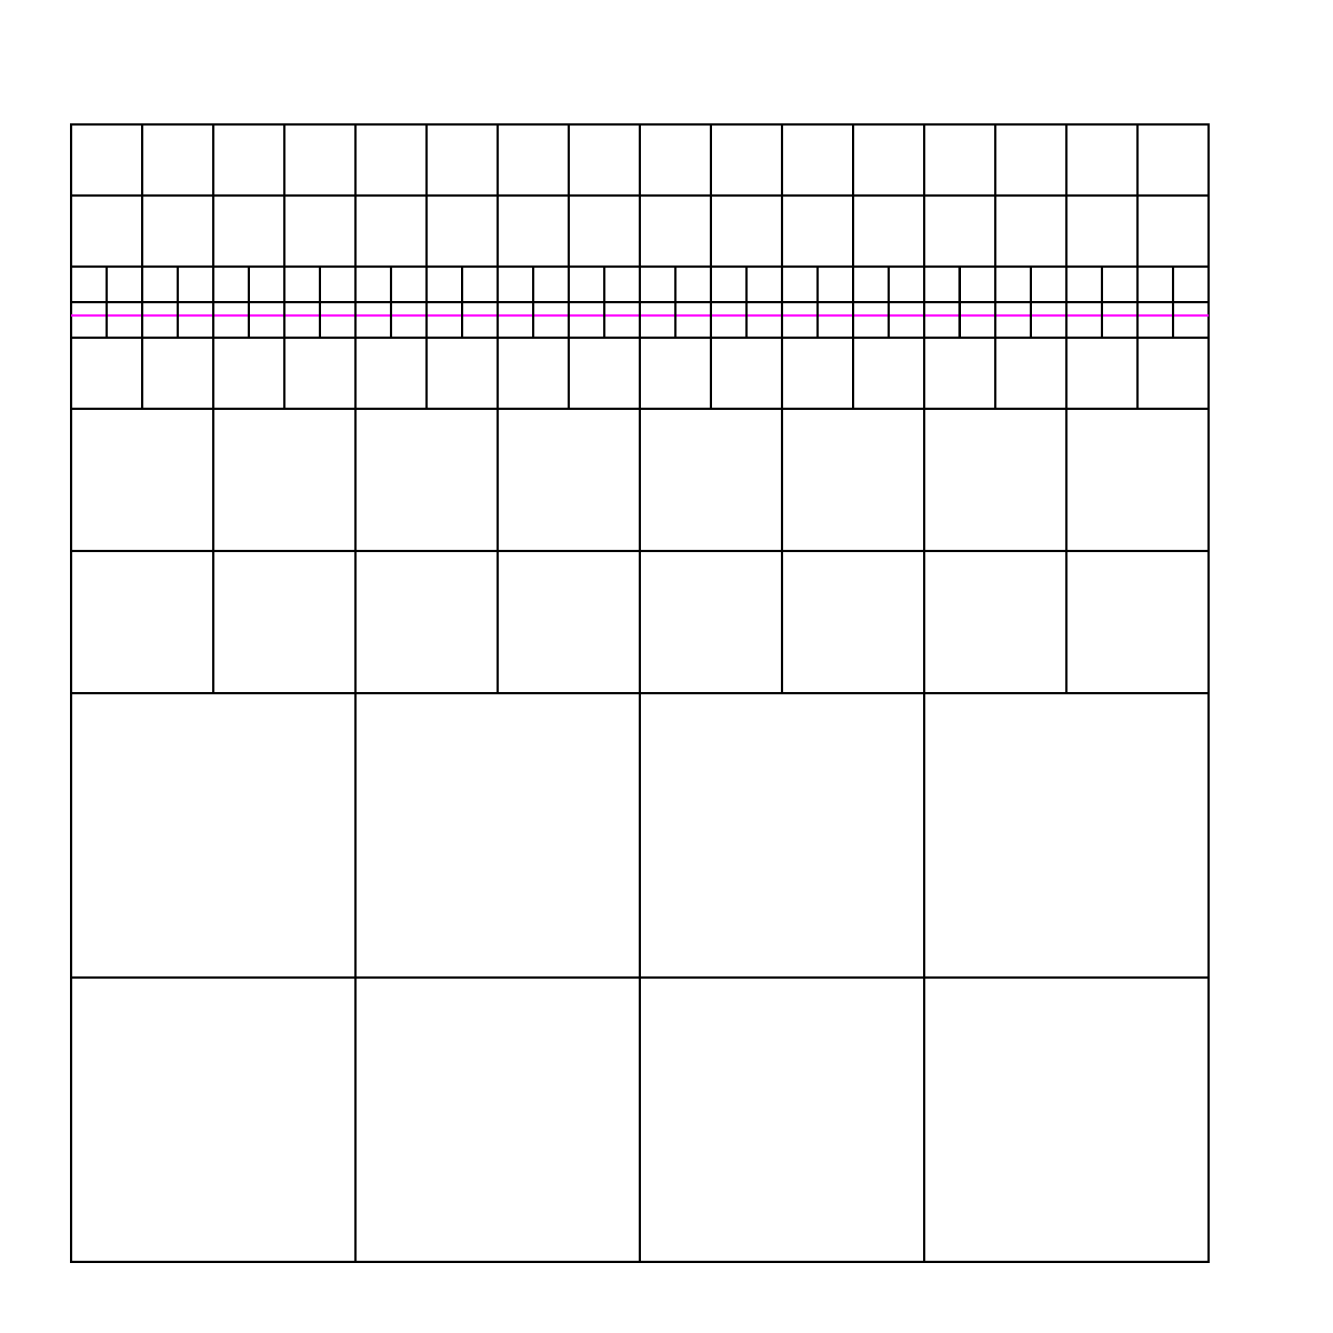
\includegraphics[width=4cm]{images/meshes/AMR/amr_5}
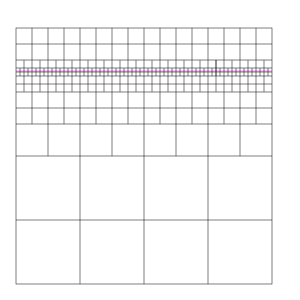
\includegraphics[width=4cm]{images/meshes/AMR/amr_6}
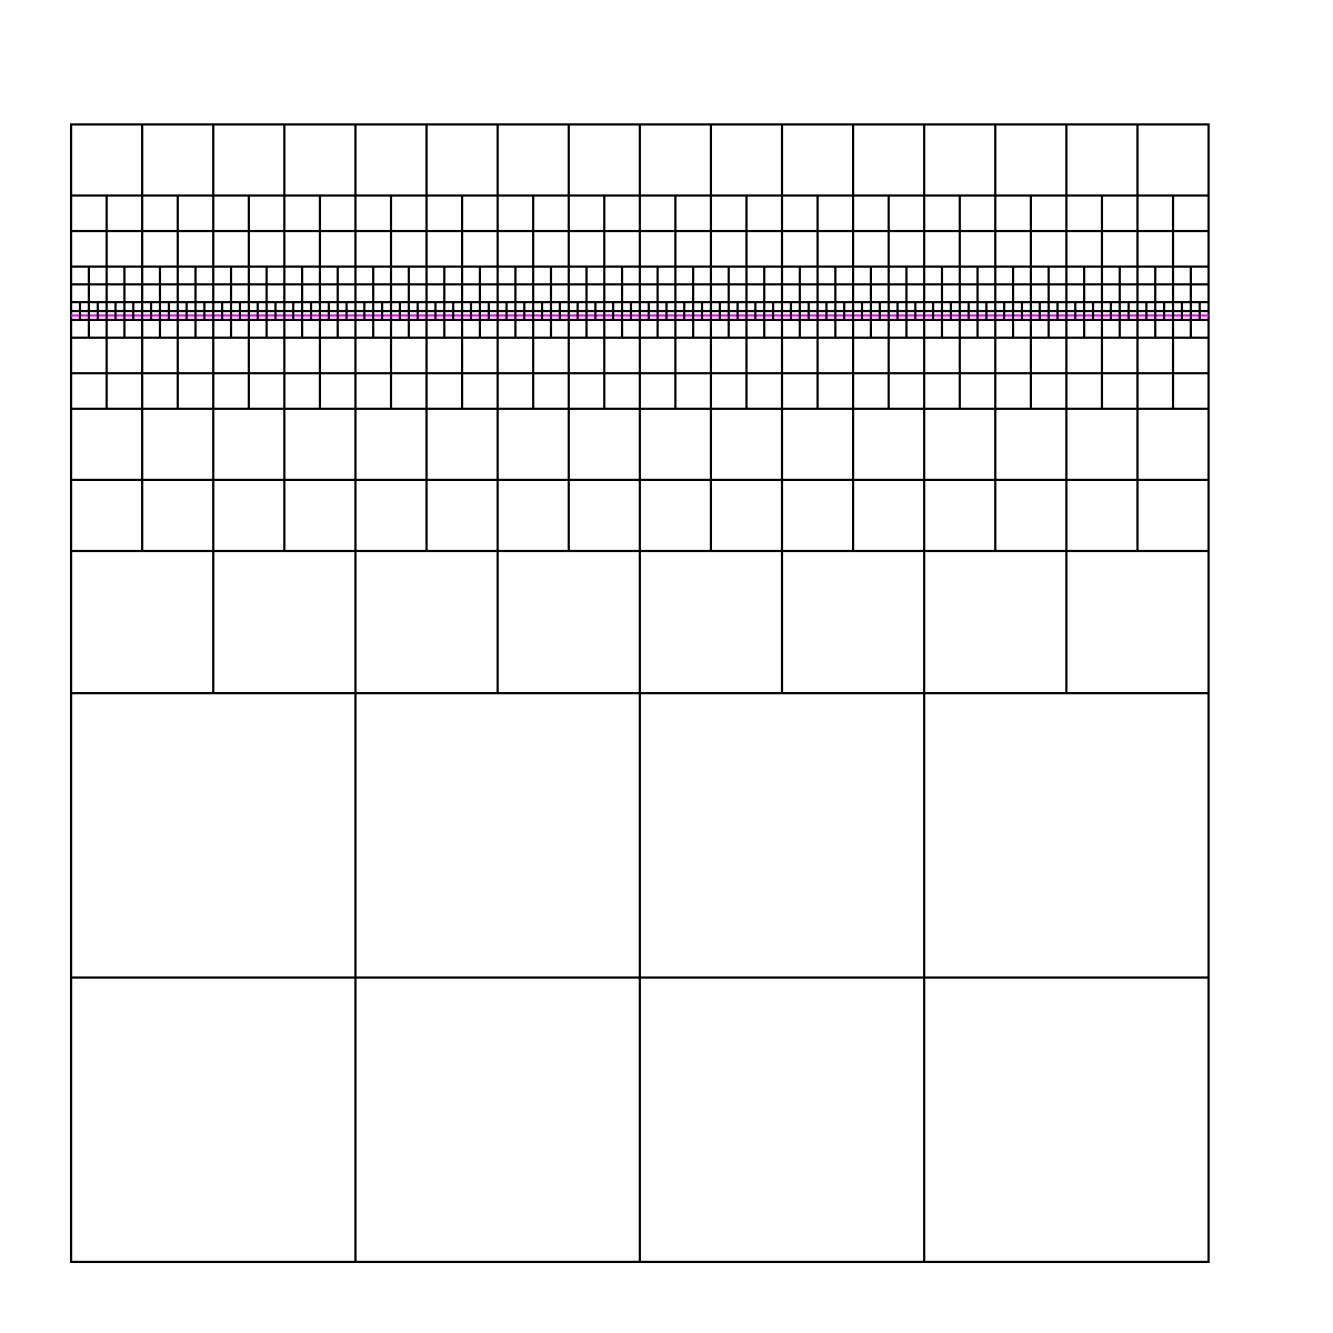
\includegraphics[width=4cm]{images/meshes/AMR/amr_7}


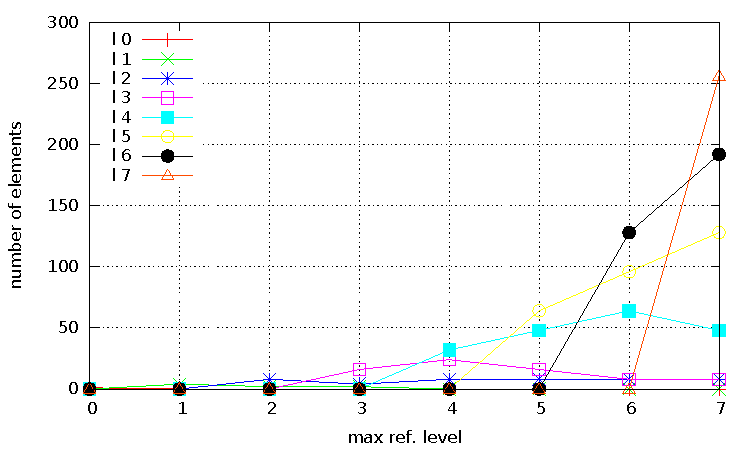
\includegraphics[width=5cm]{images/meshes/AMR/amr_data3.pdf}
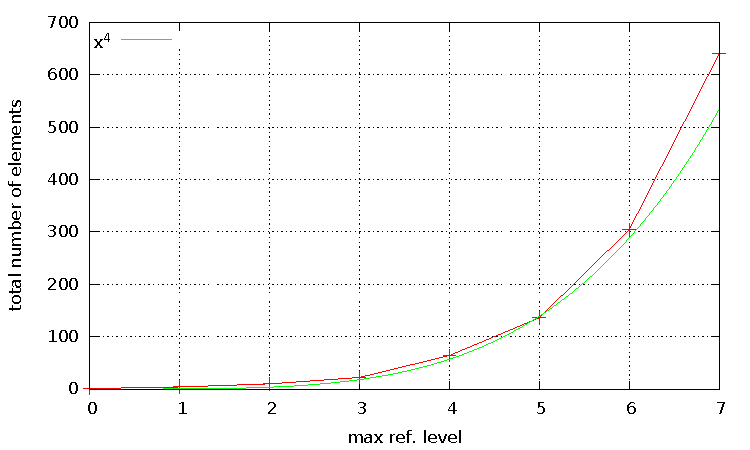
\includegraphics[width=5cm]{images/meshes/AMR/amr_data4.pdf}
\includegraphics[width=5cm]{images/meshes/AMR/amr_data5.pdf}






%.......................................
\subsubsection{Conformal Mesh Refinement \label{ss:cmr}}
\index{general}{Conformal Mesh Refinement}

The quadtree/octree mesh refinement presented above is one option
when it comes to mesh refinement (or $h$-refinement). However their 
massive drawback is the presence of hanging notes which require 
special attention. 
Another approach to mesh refinement is conformal mesh refinement
as best exemplified on the following figures: 

\begin{center}
\includegraphics[height=4.5cm]{images/meshes/amrnew}\\
{\captionfont Taken from Deb \etal (1996) \cite{depl96}.
A typical instance of the outcome of the refinement procedure. 
Notice that the `spill-over' is reduced to one row on each side of the `localized' elements.}
\end{center}

\begin{center}
\includegraphics[height=4.5cm]{images/meshes/vaks15}
\includegraphics[height=4.5cm]{images/meshes/depl96}
\includegraphics[height=4.5cm]{images/meshes/habo04}\\
\includegraphics[height=4.5cm]{images/meshes/kott05}
\includegraphics[height=4.5cm]{images/meshes/specfem}\\
\includegraphics[height=4.5cm]{images/meshes/conf3D}\\
{\captionfont 
Top row, From left to right: 
van Driel \etal (2015) \cite{vaks15}; 
Deb \etal (1996) \cite{depl96}; 
Harris \etal (2004) \cite{habo04}; 
Komatitsch \etal (2005) \cite{kott05}; 
Middle row: Specfem manual;
Bottom row: I don't know anymore.}
\end{center}

\begin{center}
\includegraphics[height=5cm]{images/meshes/gari09_a}
\includegraphics[height=5cm]{images/meshes/gari09_b}\\
{\captionfont Taken from Garimella (2009) \cite{gari09}.}
\end{center}

\begin{center}
\includegraphics[height=4cm]{images/meshes/newmeshref1}
\includegraphics[height=4cm]{images/meshes/newmeshref2}
\end{center}


\begin{center}
\includegraphics[height=4cm]{images/meshes/refine_mesh_sheet_directional1}
\includegraphics[height=4cm]{images/meshes/refine_mesh_sheet_directional2}
\includegraphics[height=4cm]{images/meshes/refine_mesh_sheet_directional4}\\
\url{https://cubit.sandia.gov/public/14.0/help_manual/WebHelp/mesh_generation/mesh_modification/mesh_refinement.htm}
\end{center}

\Literature: 
D{\"u}ster \& Rank \cite{dura01},
Harris \etal (2004) \cite{habo04},
Anderson \etal (2009) \cite{anbo09},
Anderson \cite{ande09}, 
Garimella (2009) \cite{gari09},
Nicolas \& Fouquet (2013) \cite{nifo13,nifo13b}.
Parrish \cite{parr07}, 
Schneiders \cite{schn00,schn96,schn96b,schn99},
Schneiders \etal \cite{scde95},
Staten \& Canann \cite{stca97},
book by Ramm \etal \cite{rarr03}.


%.......................................
\subsubsection{Stretching the mesh}

In some cases the topology of the mesh can be regular but one can for instance stretch 
the mesh such that (for instance) the vertical resolution is higher at the top than at the bottom, 
or higher in the middle than on the sides.

The idea behind the transformation is a piecewise-linear function which maps [0,L] to [0,L] where 
$L$ is the length of the domain in the $x$-direction. For instance, this transformation can take the following form:

\begin{center}
\includegraphics[width=8cm]{images/meshes/stretching/stretch_towards_center}\\
{\captionfont Parameters $\beta_1$ and $\beta_2$ control the shape of the lines.\\ 
The kinks in the line occur at $\beta_1 L$ and $(1-\beta_1)L$ (see code here under).}
\end{center}

The (minimal) code to transform the mesh is as follows:
\begin{lstlisting}
def stretch_towards_center(x,L,beta1,beta2):
    if x<beta1*L: 
       val = beta2/beta1*x
    elif x<(1.-beta1)*L: 
       val = (1-2*beta2)/(1-2*beta1)*(x-beta1*L)+beta2*L
    else:
       val=beta2/beta1*(x-(1-beta1)*L)+(1-beta2)*L
    return val

[...]

beta1=0.25
beta2=0.375

for i in range(0,NV):
    x[i]=stretch_towards_center(x[i],Lx,beta1,beta2)
\end{lstlisting}

The following meshes count 64x16 elements. The top one is a regular mesh, with square elements, 
while the second one has been stretched by means of the transformation above:

\begin{center}
\includegraphics[width=8cm]{images/meshes/stretching/stretch_x}
\end{center}

Concerning the stretching towards the top of the model domain, the transformation line is as follows:

\begin{center}
\includegraphics[width=8cm]{images/meshes/stretching/stretch_towards_top}\\
{\captionfont Parameters $\beta_1$ and $\beta_2$ control the shape of the lines. The kinks in the 
line occur at $\beta_1 L$ and $(1-\beta_1)L$.\\ The slope of the left line is $\beta_2/\beta_1 x$.}
\end{center}

The (minimal) code to transform the mesh is as follows:
\begin{lstlisting}
def stretch_towards_top(x,L,beta1,beta2):
    if x<beta1*L: 
       val=beta2/beta1*x
    else:
       val=(1-beta2)/(1-beta1)*(x-beta1*L)+beta2*L
    return val

[...]

beta1=0.25
beta2=0.5
for i in range(0,NV):
    y[i]=stretch_towards_top(y[i],Ly,beta1,beta2)
\end{lstlisting}


The following meshes count 64x16 elements. The top one is a regular mesh, with square elements, 
while the second one has been stretched by means of the transformation above.
\begin{center}
\includegraphics[width=8cm]{images/meshes/stretching/stretch_y}
\end{center}

Finally both transformations can be applied to the same mesh:
\begin{center}
\includegraphics[width=8cm]{images/meshes/stretching/stretch_xy}
\end{center}

This approach is used in \stone 67.

%.......................................
\subsubsection{Meshes in an annulus}


\begin{center}
\includegraphics[width=6.8cm]{images/meshes/brhv08}
\includegraphics[width=6.8cm]{images/meshes/brva07a}\\
{\captionfont The quadratic finite element mesh as used in 
Brandenburg \etal \cite{brhv08,brva07a}}
\end{center}


%.......................................
\subsubsection{Meshes in/on a hollow sphere}

The following is for the most part published in Thieulot (2018) \cite{thie18}.

To a first approximation the Earth is a sphere: the Earth's polar diameter is 
about 43 kilometers shorter than its equatorial diameter, a negligible difference of 
about 0.3\%. As a consequence, modelling physical processes 
which take place in the planet require the discretisation of a sphere. 
Furthermore, because core dynamics occur on vastly difference time scales than mantle dynamics, mantle 
modelling usually leaves the core out, thereby requiring simulations to be run on a hollow sphere mesh
(with the noticeable exception of \cite{geyu07}).

Although so-called latitude-longitude grids would seem appealing, 
they suffer from the convergence of meridians at the poles
(resulting in over sampling at poles) and the juxtaposition of triangles 
near the poles and quadrilaterals elsewhere. 
As a consequence more regular, but more complex, grids have been designed 
over the years which tesselate the surface of the 
sphere into triangles or quadrilaterals (sometimes overlapping).
There is the 'cubed sphere' \cite{roip96,heta03,chob05,sthh06,chcc07,brmw10,yiym19},
the Yin-Yang grid \cite{kasa04,yoka04,yoka06,kaks08,tack08,crta14,crta16},
the Yin-Yang-zhong grid \cite{haka16}, the Yin-yang grid of 
Shahnas \& Peltier \cite{shpe15}, the spiral grid \cite{hust08}, 
an icosahedron-based grid \cite{bafr85,tasu01},
or a grid composed of 12 blocks further subdivided into quadrilaterals \cite{zhzm00} 
as used in the CitcomS code.
Note that \cite{oldp12} have also presented a method for generating a numerical 
grid on a spherical surface which 
allows the grid to be based on several different regular polyhedrons (including octahedron, 
cube, icosahedron, and rhombic dodecahedron). 
Ideally, one wishes to generate a mesh that is regular,
i.e. angles between edges/faces as close to $90^\circ$ as possible, 
of approximately similar volumes.


\begin{center}
\includegraphics[width=12cm]{images/meshes/kaks08}\\
{\captionfont Example of Yin-Yang grid. Taken from Kameyama \etal (2008) \cite{kaks08}.}
\end{center}

How such meshes are built is often not discussed in the literature. It is 
a tedious exercise of three-dimensional geometry and it can be time-consuming, especially 
the connectivity array generation. In Thieulot (2018) \cite{thie18} I present an open source 
mesh generator for three hollow sphere meshes: the 'cubed sphere' mesh, the CitcomS mesh and the 
icosahedral mesh:

\begin{itemize}
\item 
The cubed sphere ('HS06'), composed of 6 blocks which 
are themselves subdivided into $N_b \times N_b$ quadrilateral shaped cells  \cite{sado72,roip96,heta03,busa13}.
Four types of cubed spheres meshes have been proposed: the conformal, elliptic, gnomonic and spring types \cite{puli07}:


\begin{center}
\includegraphics[width=6.5cm]{images/meshes/puli07}
\includegraphics[width=8.5cm]{images/meshes/cubed_nair}\\
{\captionfont 
Left: The cubed-sphere grids at $2^\circ$ resolution displaying cells on the sphere,
 the image focuses on the distribution of grid cells near one corner of the grid;
 (a) conformal mapping \cite{rapm96,mcgr96}, (b) the gnomonic grid modified by elliptic solver,
 (c) equiangular gnomonic mapping and (d) the gnomonic grid modified by spring dynamics. \cite{puli07}.
Right: Taken from presentation by R. Nair, see Nair2008.pdf
}
\end{center}

However only gnomonic meshes are considered in Thieulot (2018): these 
are obtained by inscribing a cube within a sphere and expanding to the surface
of the sphere.
The cubed sphere has been used in large-scale mantle convection simulation in conjunction with 
Adaptive Mesh Refinement \cite{algs12,busa13}.  

\begin{center}
\includegraphics[width=4cm]{images/ghost/hs06}
\end{center}



\item 
The CitcomS mesh ('HS12') composed of 12 blocks also subdivided 
into $N_b \times N_b$ quadrilateral shaped cells
\cite{zhzm00,sthh06,zhmt08,arfw14}.
Note that \aspect{} \cite{krhb12,hedg17}, a relatively new code aimed at 
superseeding CitcomS can generate and use 
this type of mesh \cite{thie17} but is not limited to it.

\begin{center}
\includegraphics[width=4cm]{images/ghost/citcom12}
\end{center}


\item The icosahedral mesh ('HS20') composed of 20 triangular blocks \cite{bafr85,baum85} subdivided into triangles, which is 
used in the TERRA code \cite{burb96,burb97,burl98,dadb13}.
\end{itemize}


\begin{center}
\includegraphics[width=8cm]{images/meshes/spherical_choices1}
\includegraphics[width=8cm]{images/meshes/spherical_choices2}\\
{\captionfont source?}
\end{center}



Given the regularity and symmetry of these meshes determining the location of the 
mesh nodes in space is a relatively straightforward task. Building the mesh connectivity in an 
efficient manner is where the difficulty lies.

The approach to building all three meshes is identical:
\begin{enumerate}
\item A reference square or triangle is populated with cells,
parametrised by a level $l$: the square is subdivided into $l\times l$ quadrilaterals while 
the triangle is subdivided into $l^2$ triangles.
\begin{center}
\includegraphics[width=8cm]{images/ghost/f01_basics}\\
{\captionfont Reference square and triangles meshes at level 5.}
\end{center}

\item This reference square or triangle is then replicated {\sl nblock} times (6, 12 or 20) and mapped
onto a portion of a unit sphere. The blocks are such that their union covers a full sphere
but they cannot overlap except at the edges:
\begin{center}
\includegraphics[width=.8\linewidth]{images/ghost/f02}\\
{\captionfont From left to right: HS06, HS12 and HS20 shells coloured by block number.}
\end{center}

\item All block meshes are then merged together to generate a shell mesh. This task is rather 
complex as duplicate nodes must be removed and all connectivity arrays of the blocks must then 
be mended accordingly. 

\item Shell meshes are replicated {\sl nlayer+1} times outwards with increasing radii. 
The {\sl nlayer} shells are then merged together to form a hollow sphere mesh:
\begin{center}
\includegraphics[width=10cm]{images/ghost/f03_3HS}\\
{\captionfont a) HS06 mesh composed of 6 blocks containing each $6^3$ cells; 
b) HS12 mesh composed of 12 blocks containing each 
$6^3$ cells; e) HS20 mesh composed of 20 blocks containing each $6^3$ cells.}
\end{center}

\end{enumerate}



More information on these steps is available in the manual of the code.
In the following table the number of nodes and cells for a variety of resolutions 
for all three mesh types is reported. Looking at the CitcomS literature of the past 20 years, we find that 
the mesh data presented in this table cover the various resolutions used, e.g.
$12\times48^3$ \cite{mczh04,arfw14}, $12\times64^3$ \cite{budt14}
$12\times96^3$ \cite{bumb10}, $12\times128^3$ \cite{beck06,wele16,welm16}.
Note that in the case of the HS06 and HS12 meshes the mesh nodes are mapped out to the 6 or 12 blocks 
following either an equidistant or equiangle approach (see \cite{puli07}
for details on both approaches). 

\begin{center}
\begin{tabular}{lrrrl}
\hline
type & level & $N$ & $N_{el}$ & structure\\
\hline
\hline
HS06 & 
2   &  78        &  48         &$6\times 2^3$    \\
HS06 & 
4   &  490       &  384        &$6\times 4^3$    \\
HS06 & 
8   &  3,474      &  3,072       &$6\times 8^3$    \\
HS06 & 
16  &  26,146     &  24,576      &$6\times 16^3$    \\
HS06 & 
32  &  202,818    &  196,608     &$6\times 32^3$    \\
HS06 & 
64  &  1,597,570   &  1,572,864    &$6\times 64^3$    \\
HS06 & 
128 &  12,681,474  &  12,582,912   &$6\times 128^3$    \\
HS06 & 
256 &  101,057,026 &  100,663,296  &$6\times 256^3$    \\
\hline
HS12 & 2    &          150  &          96  &  $12\times 2^3$ \\
HS12 & 4    &          970  &         768  &  $12\times 4^3$ \\
HS12 & 8    &        6,930  &       6,144  &  $12\times 8^3$ \\
HS12 & 16   &       52,258  &      49,152  &  $12\times 16^3$ \\
HS12 & 32   &      405,570  &     393,216  &  $12\times 32^3$ \\
HS12 & 48   &    1,354,850  &   1,327,104  &  $12\times 48^3$ \\
HS12 & 64   &    3,195,010  &   3,145,728  &  $12\times 64^3$ \\
HS12 & 128  &   25,362,690  &  25,165,824  &  $12\times 128^3$ \\
HS12 & 256  &  202,113,538  & 201,326,592  &  $12\times 256^3$ \\
\hline
HS20 & 
2     &         126  &         160   & $20 \times 2^3$ \\
HS20 & 
4     &         810  &       1,280   & $20 \times 4^3$ \\
HS20 & 
8     &       5,778  &      10,240   & $20 \times 8^3$ \\
HS20 & 
16    &      43,554  &      81,920   & $20 \times 16^3$ \\
HS20 & 
32    &     337,986  &     655,360   & $20 \times 32^3$ \\
HS20 & 
64    &   2,662,530  &   5,242,880   & $20 \times 64^3$ \\
HS20 & 
128   &  21,135,618  &  41,943,040   & $20 \times 128^3$ \\
HS20 & 
256   & 168,428,034  & 335,544,320   & $20 \times 256^3$ \\
\hline
\end{tabular}\\
{\captionfont Number of nodes $N$ and elements/cells $N_{el}$ for the three types of meshes and for various 
levels.\\ HS06: cubed sphere; HS12: CitcomS mesh; HS20: icosahedral mesh.}
\end{center}

There are also many possibilities offered by the use of tetrahedral cells/elements:


\begin{center}
\includegraphics[height=4.5cm]{images/meshes/oebm09}
\includegraphics[height=4.5cm]{images/meshes/geotess}\\
{\captionfont Left: Grid of a global neo-tectonic SHELLS model coupled to a global mantle
circulation model; colours represent temperatures (red=hot, blue=cold)
at a depth of $200\si{km}$ below the surface. Taken from Oeser \etal (2009) \cite{oebm09}.
Right: Taken from the GeoTess software \footnote{\url{https://www.sandia.gov/geotess/}} manual.}
\end{center}


\begin{center}
\includegraphics[width=7cm]{images/meshes/htm}\\
{\captionfont Example of a Hierarchical Triangular Mesh}
\end{center}


\begin{center}
\includegraphics[width=7cm]{images/meshes/bafr85}
\includegraphics[width=7cm]{images/meshes/simj12}\\
{\captionfont \textcite{bafr85} (1985), \textcite{simj12} (2012)}
\end{center}


\Literature: Phillips \etal \cite{phdo19} present an algorithm which builds polyhedral-based grids.
\textcite{upsm11} (2011) on icosahedral-hexagonal grids on a sphere for CFD applications.
\textcite{saku97} (1997) on distributing many points on a sphere.
\textcite{swpu06} on Fibonacci grids which possess virtually uniform and isotropic resolution, 
with an equal area for each grid point.
\textcite{hasa04} on discretizing manifolds via Minimum Energy Points.



